\documentclass{ctexart}
\usepackage{amsmath}
\usepackage{rotating}
\usepackage{xparse,tikz}
\usetikzlibrary{calc}
\usepackage[margin = 2cm]{geometry}
\setlength{\emergencystretch}{4em}
\usepackage{graphicx}
\usepackage{subcaption}
\usepackage{zhnumber}
\usepackage{float} 

\NewDocumentCommand{\makecover}{}{
  \begin{titlepage}
  \begin{center}
  \vspace*{5cm}
  {\LARGE\bfseries 电磁场与电磁波}\par
  \vspace{1.5cm}
  {\Large\bfseries 矩形波导馈电角锥喇叭天线 CST 仿真}\par
  \vspace{1cm}
  {\large 实验报告}
  \end{center}
  \end{titlepage}
}

\NewDocumentCommand{\makecoveri}{}{
  \begin{center}
  \begin{minipage}[c][145pt][c]{\textwidth}
  \centering{\Large\bfseries 电磁场与电磁波}\par
  \vspace{1cm}
  {\large 矩形波导馈电角锥喇叭天线 CST 仿真}
  \end{minipage}
  \end{center}
}

\newcounter{makepart}
\setcounter{makepart}{1}
\NewDocumentCommand{\makepart}{+m}
{
  \vspace{1em}
  \begin{flushleft}
   \large\bfseries\zhnumber{\arabic{makepart}}、#1
  \end{flushleft} 
  \stepcounter{makepart}
}

\NewDocumentCommand{\zdx}{}
{
  \tikz[remember picture,overlay]{
    \coordinate (s) at ([shift={(1,-3)}]current page.north west);
    \coordinate (e) at ([shift={(1,3)}]current page.south west);
    \foreach \x in{0,0.15,...,9.2}
    {
      \fill[] ($(s)+(0,-\x)$) circle(1pt);
    }
    \foreach \x in{0,0.15,...,9.2}
    {
      \fill[] ($(e)+(0,\x)$) circle(1pt);
    }
    \node[text width=1em,align=center]at($(s)!0.5!(e)$){装\\[10pt]订\\[10pt]线};
  }
}

\pagestyle{empty}

\begin{document}
\makecover
\makecoveri
\zdx

\makepart{实验目的与要求}

\subsection*{1.1 实验目的}
本实验旨在通过三维电磁仿真软件的实际操作，加深对微波技术与天线理论的理解，具体目的包括：
\begin{enumerate}
    \item 了解并掌握波导喇叭天线的常用参数指标（如 $S_{11}$ 反射系数、电压驻波比 VSWR、方向图、增益等）的物理意义及理论分析方法。
    \item 熟悉 CST Studio Suite 软件的基本操作流程，掌握运用该软件对特定的微波器件或电路进行参数化建模、网格划分、端口激励设置以及仿真分析的完整工作流。
\end{enumerate}

\subsection*{1.2 实验任务与要求}
根据给定的矩形波导角锥喇叭天线尺寸参数，在 CST 软件中独立完成三维建模。完成建模后，仿真计算天线的端口阻抗匹配特性及空间辐射特性，提取核心数据，并与喇叭天线的理论增益及实际辐射特性测量实验的结果进行对比与误差分析。

具体的角锥喇叭天线及馈电波导结构尺寸要求如图 \ref{fig:antenna_dim} 所示：
\begin{itemize}
    \item \textbf{角锥喇叭天线尺寸}：$D_H = 80\,\text{mm}$，$D_E = 38\,\text{mm}$，$L = 80\,\text{mm}$。
    \item \textbf{波导尺寸}：$a = 22.86\,\text{mm}$，$b = 10.16\,\text{mm}$，中心频率波长 $\text{Lambda} = 29.1\,\text{mm}$。
    \item \textbf{铜壁厚度}：$t = 1\,\text{mm}$。
\end{itemize}

\begin{figure}[htbp]
    \centering
    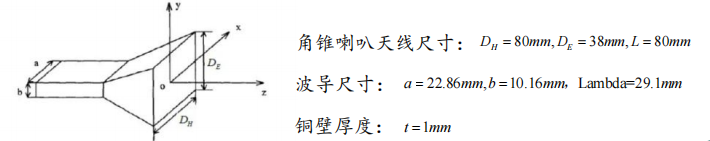
\includegraphics[width=0.85\textwidth]{figures/antenna_dim.png}
    \caption{角锥喇叭天线结构及具体尺寸参数}
    \label{fig:antenna_dim}
\end{figure}

\makepart{实验原理}

\subsection*{2.1 喇叭天线概述}
喇叭天线是一种在微波频段应用极为广泛的开口源天线。其主要优点在于结构简单、频带宽、功率容量大且易于调整。通过合理设计喇叭的几何尺寸，可以获得极佳的辐射特性，如较窄的主瓣宽度、极低的副瓣电平以及较高的定向增益。因此，喇叭天线不仅在军用雷达和民用通信中被大量使用，更常被用作天线测量实验中的标准测试天线。

从物理本质上看，喇叭天线是由矩形或圆形波导的开口面逐渐向外扩展平滑过渡而成的。这种渐变扩展的结构相当于一个阻抗变换器，极大地改善了波导特性阻抗与自由空间波阻抗（$377\,\Omega$）之间的匹配情况。这种设计有效降低了波导端口的电压反射系数，使得波导中传输的电磁波能量能够最大程度地向自由空间辐射。

根据波导截面形状及扩展方式的不同，喇叭天线主要分为以下几类：
\begin{itemize}
    \item \textbf{矩形波导馈电的喇叭天线}：根据扩展面的不同，分为由窄边扩展而成的 E 面扇形喇叭、由宽边扩展而成的 H 面扇形喇叭，以及宽、窄边同时扩展的角锥喇叭（如图 \ref{fig:rect_horn} 所示）。本实验采用的即为矩形波导馈电的角锥喇叭天线。
    \item \textbf{圆波导馈电的喇叭天线}：通常为圆锥喇叭，其电磁场模式由圆波导模式平滑过渡而来（如图 \ref{fig:circ_horn} 所示）。
\end{itemize}

\begin{figure}[htbp]
    \centering
    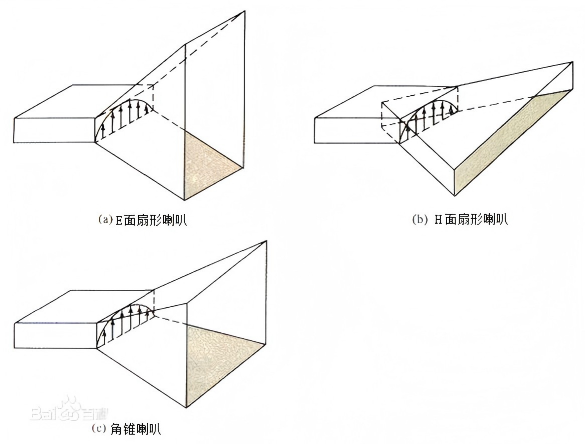
\includegraphics[width=0.85\textwidth]{figures/三种矩形波导馈电角锥喇叭天线的结构示意图.png}
    \caption{三种矩形波导馈电的喇叭天线示意图}
    \label{fig:rect_horn}
\end{figure}

\begin{figure}[htbp]
    \centering
    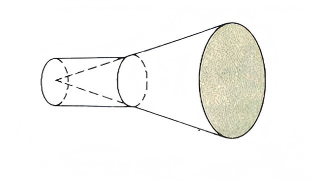
\includegraphics[width=0.45\textwidth]{figures/圆波导馈电圆锥喇叭天线结构示意图.png}
    \caption{圆波导馈电圆锥喇叭天线结构示意图}
    \label{fig:circ_horn}
\end{figure}

\subsection*{2.2 喇叭天线的几何结构}
角锥喇叭天线是由馈电矩形波导在 H 面（xz 面，即宽边平行面）和 E 面（yz 面，即窄边平行面）按一定张角同时展开形成的。其核心几何参数如图 \ref{fig:horn_geo} 所示。

设馈电矩形波导的内部尺寸为 $a \times b$（$a$ 为宽边，$b$ 为窄边），喇叭辐射口径尺寸为 $D_H \times D_E$，喇叭渐变段的高度为 $L$。在几何关系上，展开面延长线会交于一点（即虚顶点）。其中，H 面内虚顶点到口径中心的垂直距离记为 $R_1$；E 面内虚顶点到口径中心的垂直距离记为 $R_2$。在实际的完美角锥喇叭设计中，通常要求这两个虚顶点重合以保证相位的均匀性。

\begin{figure}[htbp]
    \centering
    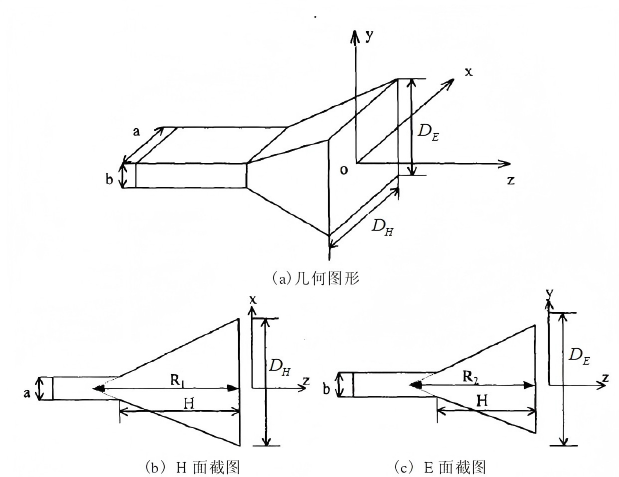
\includegraphics[width=0.8\textwidth]{figures/角锥喇叭天线的结构示意图.png}
    \caption{角锥喇叭天线的几何图形及截面参数图}
    \label{fig:horn_geo}
\end{figure}

\subsection*{2.3 角锥喇叭天线的增益理论计算}
角锥喇叭天线的增益取决于其口径面积以及口径面上的电磁场相位分布。对于尺寸为 $a \times b$，口径面积 $A^2 = D_H \times D_E$，高度为 $L$ 的角锥喇叭，其实际增益 $G$ 可由以下半经验公式估算：
\begin{equation}
    G = 10.8 + 10\lg\left(\frac{D_H \times D_E}{\lambda^2}\right) - \Delta G_H - \Delta G_E \quad (\text{dB})
\end{equation}

公式中，$10.8 + 10\lg(\frac{D_H \times D_E}{\lambda^2})$ 为假设口径面相位完全均匀时的理想增益。而 $\Delta G_H$ 和 $\Delta G_E$ 分别代表由于 H 面和 E 面展开导致口径面存在球面相位差而引起的增益衰减因子。这两个衰减参数 $\Delta G_H, \Delta G_E$ 可通过查阅标准数值表获得，查表所需的中间变量 $\alpha$ 和 $\beta$ 的推导公式如下：

首先，根据相似三角形原理计算虚顶点距离 $R_1$ 和 $R_2$：
\begin{equation}
    R_1 = \frac{L \times D_H}{D_H - a}
\end{equation}
\begin{equation}
    R_2 = \frac{L \times D_E}{D_E - b}
\end{equation}

计算喇叭壁的斜面长度 $L_H$ 和 $L_E$：
\begin{equation}
    L_H = \sqrt{R_1^2 + \frac{D_H^2}{4}}
\end{equation}
\begin{equation}
    L_E = \sqrt{R_2^2 + \frac{D_E^2}{4}}
\end{equation}

依据相差因子计算参数 $S_H$ 和 $S_E$：
\begin{equation}
    S_H = \frac{A^2}{8\lambda L_H}
\end{equation}
\begin{equation}
    S_E = \frac{A^2}{8\lambda L_E}
\end{equation}

最终得到用于查表的自变量 $\alpha$ 和 $\beta$：
\begin{equation}
    \alpha = 8S_H
\end{equation}
\begin{equation}
    \beta = 8S_E
\end{equation}

求得 $\alpha$ 和 $\beta$ 后，查表获取对应的 $\Delta G_H$ 和 $\Delta G_E$，代入式 (1) 即可求得该角锥喇叭天线在特定工作频率（波长 $\lambda$）下的理论增益值。

\makepart{CST 仿真与建模步骤}

\subsection*{3.1 CST 初始环境设置}
在进行天线三维建模与仿真前，首先需要配置 CST Studio Suite 的工作环境及求解器类型。具体初始化步骤如下：
打开 CST 软件，点击新建工程（New Project），依次选择微波与射频模块（MICROWAVES \& RF） $\rightarrow$ 天线（Antennas） $\rightarrow$ 波导天线（Waveguide: Horn, Cone, etc.）。在求解器选择界面，选择时域求解器（Time Domain）。最后，在单位设置界面，将几何尺寸单位设置为毫米（Dimensions: mm），频率单位设置为吉赫兹（Frequency: GHz），完成初始工程模板的建立。

\subsection*{3.2 角锥喇叭天线的三维建模过程}

\subsubsection*{3.2.1 建模参数初始化}
为了方便后续的模型尺寸修改、优化以及参数扫描，本实验采用\textbf{参数化建模}的方式。在正式绘制三维几何体之前，首先在 CST 界面下方的参数列表（Parameter List）中定义所有需要用到的结构变量。

根据本次实验的具体任务要求，角锥喇叭天线及馈电矩形波导的各项尺寸参数设定如表 \ref{tab:parameters} 所示。

\begin{table}[htbp]
    \centering
    \caption{角锥喇叭天线建模参数表}
    \vspace{5pt}
    \begin{tabular}{clc}
        \hline
        \textbf{变量名 (Parameter)} & \textbf{物理含义描述} & \textbf{设定值 (Value / mm)} \\
        \hline
        \texttt{a1} & 矩形波导宽边尺寸 & 22.86 \\
        \texttt{b1} & 矩形波导窄边尺寸 & 10.16 \\
        \texttt{Lambda} & 中心频率对应波长 & 29.1 \\
        \texttt{DH} & 喇叭口径 H 面尺寸 & 80 \\
        \texttt{DE} & 喇叭口径 E 面尺寸 & 38 \\
        \texttt{L}  & 喇叭渐变段轴向长度 & 80 \\
        \texttt{t}  & 天线铜壁厚度 & 1 \\
        \hline
    \end{tabular}
    \label{tab:parameters}
\end{table}

在 CST 软件的 Parameter List 中逐一输入上述变量及表达式后，完成的参数列表初始设置如图 \ref{fig:cst_parameters} 所示。这些变量将在后续的 Brick（长方体）绘制、Loft（放样）以及 Shell（抽壳）等建模操作中被直接调用。

\begin{figure}[htbp]
    \centering
    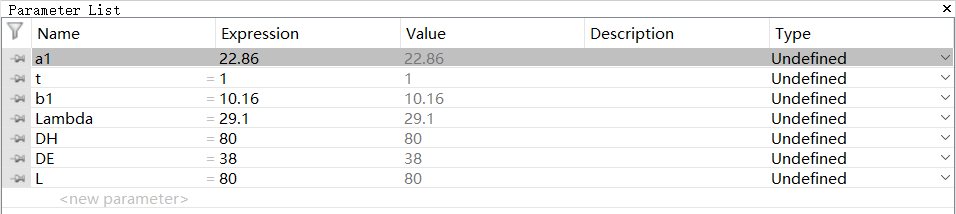
\includegraphics[width=0.9\textwidth]{figures/image_eeb23c.png}
    \caption{CST 软件中的参数列表 (Parameter List) 录入结果}
    \label{fig:cst_parameters}
\end{figure}

\subsubsection*{3.2.2 角锥喇叭天线的三维实体建模}
在完成参数定义后，按照从馈电波导到喇叭口径的顺序进行三维几何建模，具体步骤如下：

\paragraph{1. 创建馈电矩形波导}
在 \texttt{Modeling} 选项卡中选择 \texttt{Brick} 工具，调用此前设置的 \texttt{a1}、\texttt{b1} 等参数构建矩形波导的实体模型，并将其材质设定为 \texttt{PEC}（理想导体）。参数设置及生成的初步模型分别如图6、图7所示。

\begin{figure}[htbp]
    \centering
    \begin{minipage}[t]{0.48\textwidth}
        \centering
        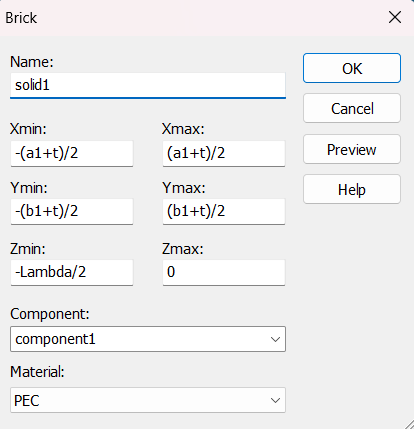
\includegraphics[width=\textwidth]{figures/矩形波导的结构参数设置图.png}
        \caption{矩形波导的结构参数设置}
    \end{minipage}
    \hfill
    \begin{minipage}[t]{0.48\textwidth}
        \centering
        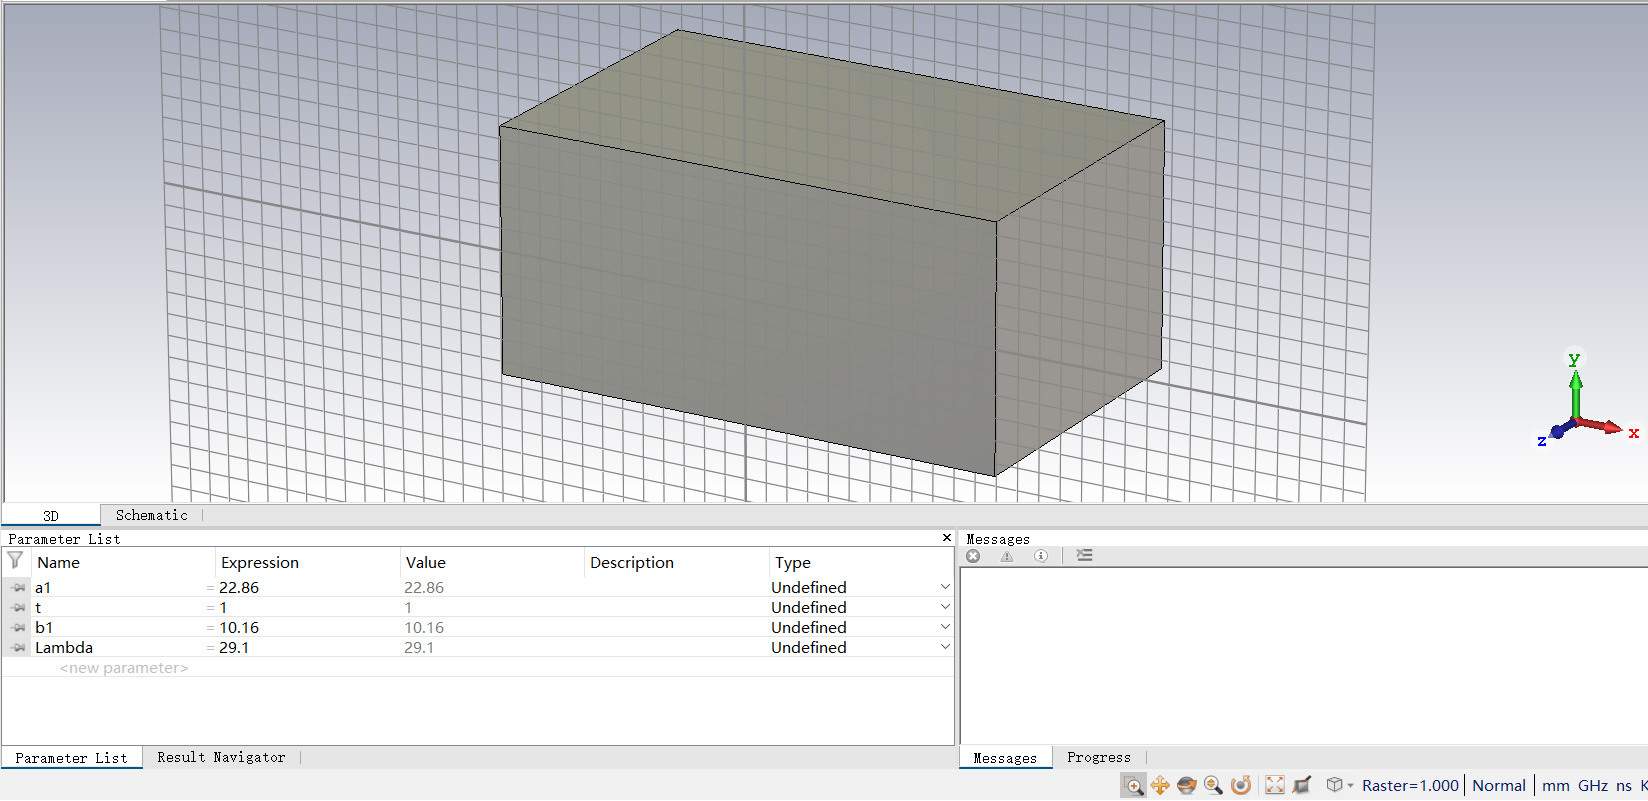
\includegraphics[width=\textwidth]{figures/矩形波导 CST 模型.png}
        \caption{矩形波导 CST 模型}
    \end{minipage}
    \label{fig:waveguide_build}
\end{figure}

\paragraph{2. 创建喇叭口径面}
利用曲线工具（Curves）绘制喇叭口径面的矩形轮廓，随后将其转化为实心面（Face），作为放样（Loft）操作的目标面，分别如图8、图9所示。

\begin{figure}[htbp]
    \centering
    \begin{minipage}[t]{0.48\textwidth}
        \centering
        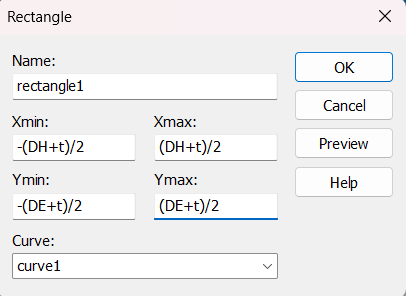
\includegraphics[width=\textwidth]{figures/曲线参数设置.png}
        \caption{喇叭口径面的曲线参数设置}
    \end{minipage}
    \hfill
    \begin{minipage}[t]{0.48\textwidth}
        \centering
        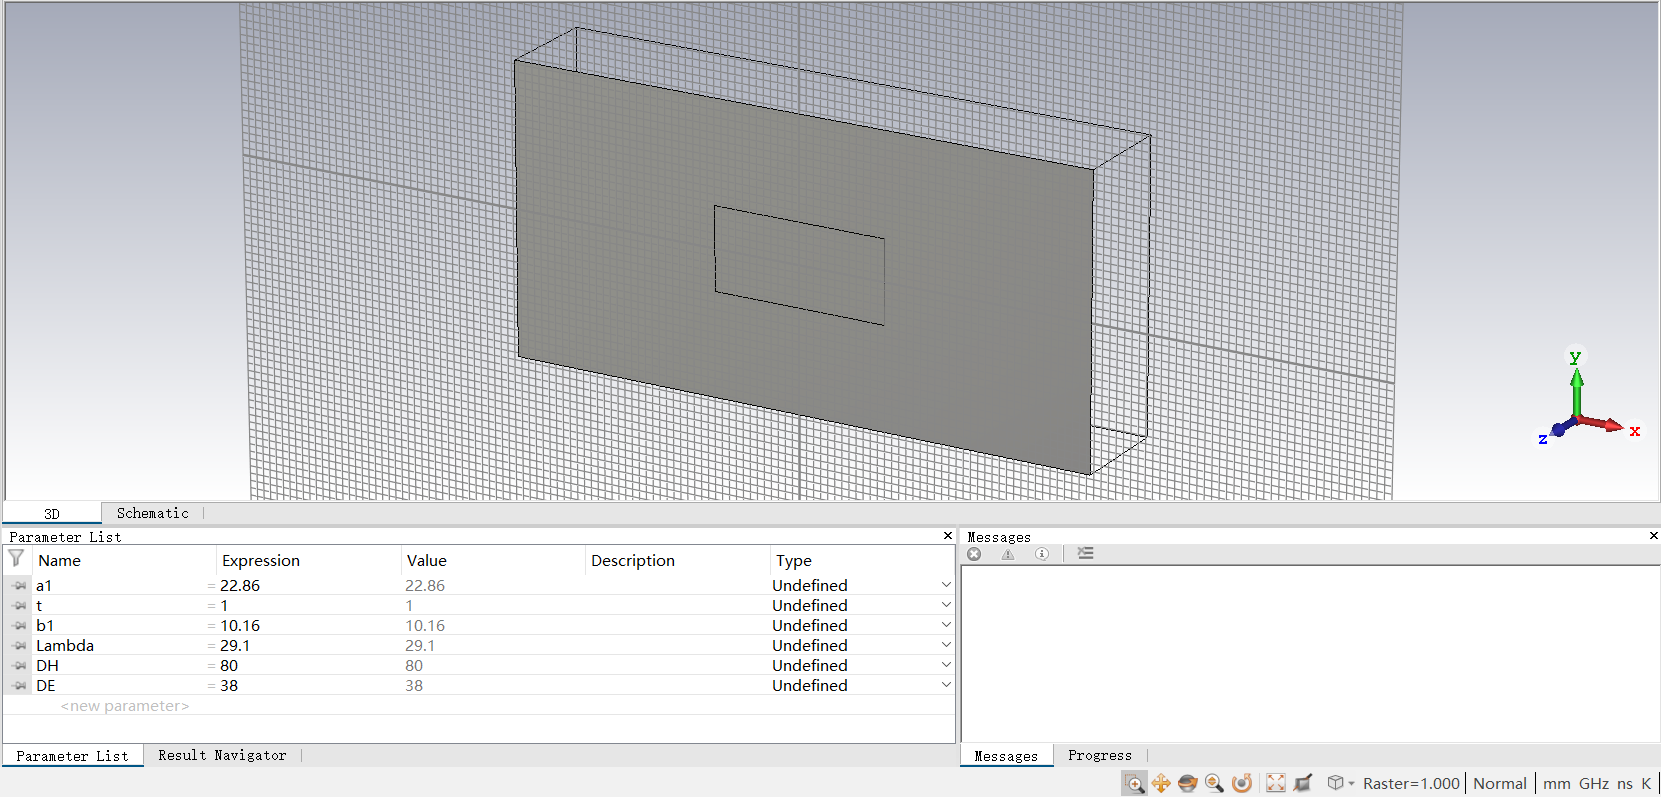
\includegraphics[width=\textwidth]{figures/喇叭口径面.png}
        \caption{生成的喇叭口径面}
    \end{minipage}
    \label{fig:aperture_create}
\end{figure}

\paragraph{3. 设置喇叭口径面的空间位置}
选中刚创建的口径面，依次点击 \texttt{Modeling -> Transform -> Translate}。在 Z 轴的平移向量（Translation vector）中输入参数 \texttt{L}，将口径面沿 Z 轴正方向推移至指定位置，分别如图10、图11所示。

\begin{figure}[htbp]
    \centering
    \begin{minipage}[t]{0.48\textwidth}
        \centering
        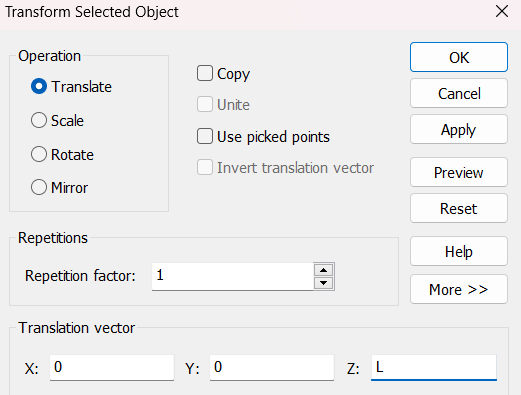
\includegraphics[width=\textwidth]{figures/设置喇叭口径面的空间位置.png}
        \caption{平移操作的参数设置}
    \end{minipage}
    \hfill
    \begin{minipage}[t]{0.48\textwidth}
        \centering
        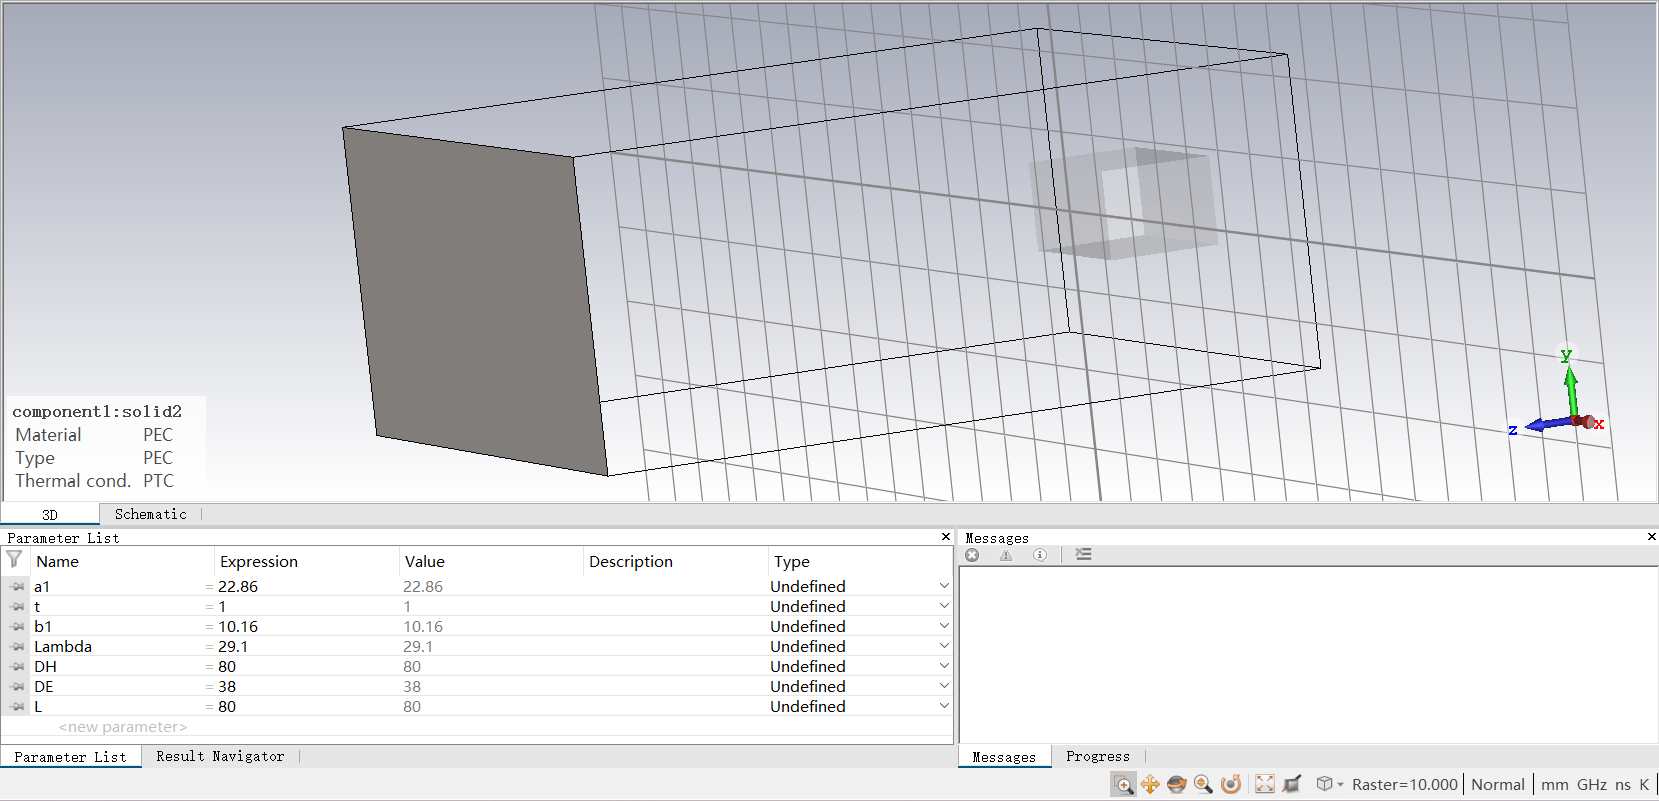
\includegraphics[width=\textwidth]{figures/喇叭口径面 CST 模型.png}
        \caption{平移后的喇叭口径面 CST 模型}
    \end{minipage}
    \label{fig:aperture_translate}
\end{figure}

\paragraph{4. 放样创建喇叭侧壁}
分别选中原矩形波导的开口端面与刚刚平移到位的喇叭口径面，使用放样命令 \texttt{Modeling -> Shapes -> Loft}，将两个面连接起来，生成实心的喇叭侧壁几何体，分别如图12、图13所示。

\begin{figure}[htbp]
    \centering
    \begin{minipage}[t]{0.48\textwidth}
        \centering
        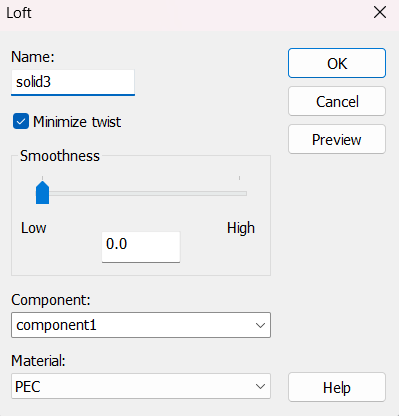
\includegraphics[width=\textwidth]{figures/Loft参数.png}
        \caption{Loft 放样操作参数设置}
    \end{minipage}
    \hfill
    \begin{minipage}[t]{0.48\textwidth}
        \centering
        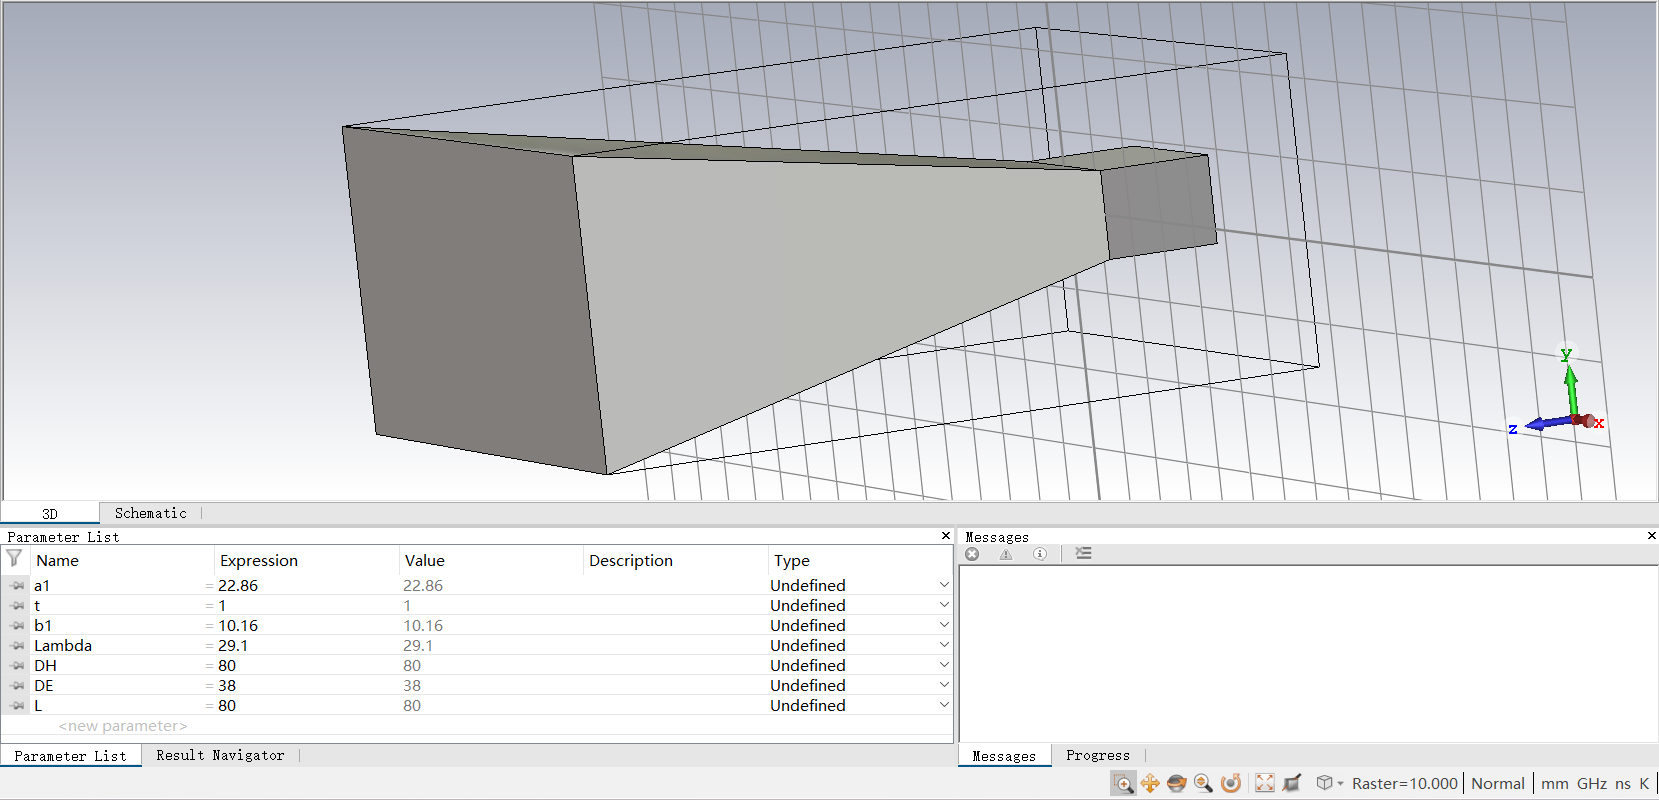
\includegraphics[width=\textwidth]{figures/喇叭侧壁的 CST 模型.png}
        \caption{生成的喇叭侧壁 CST 模型}
    \end{minipage}
    \label{fig:loft_build}
\end{figure}

\paragraph{5. 全层相加 (Boolean Add)}
为保证天线结构的连续性，使用 \texttt{Modeling -> Boolean -> Add} 命令，将矩形波导块与喇叭侧壁块进行布尔相加，使整个 PEC 结构融合为一个单一的物理对象。


\paragraph{6. 实体掏空生成最终模型}
此时的模型仍为实心块。分别选中结构前（喇叭口）、后（波导端）两个需要开口的端面，执行掏空命令 \texttt{Modeling -> Shape tools -> Shell Solid or Thicken Sheet}。在弹出的对话框中选择 \texttt{Inside}，厚度（Thickness）填入壁厚参数 \texttt{t}。执行后即可得到内部中空的角锥喇叭天线最终 CST 模型，分别如图14、图15所示。

\begin{figure}[htbp]
    \centering
    \begin{minipage}[t]{0.48\textwidth}
        \centering
        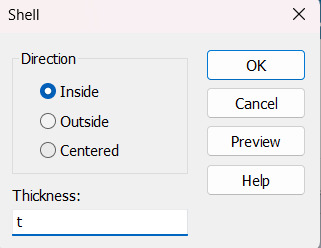
\includegraphics[width=\textwidth]{figures/掏空参数设置.png}
        \caption{Shell 掏空操作参数设置}
    \end{minipage}
    \hfill
    \begin{minipage}[t]{0.48\textwidth}
        \centering
        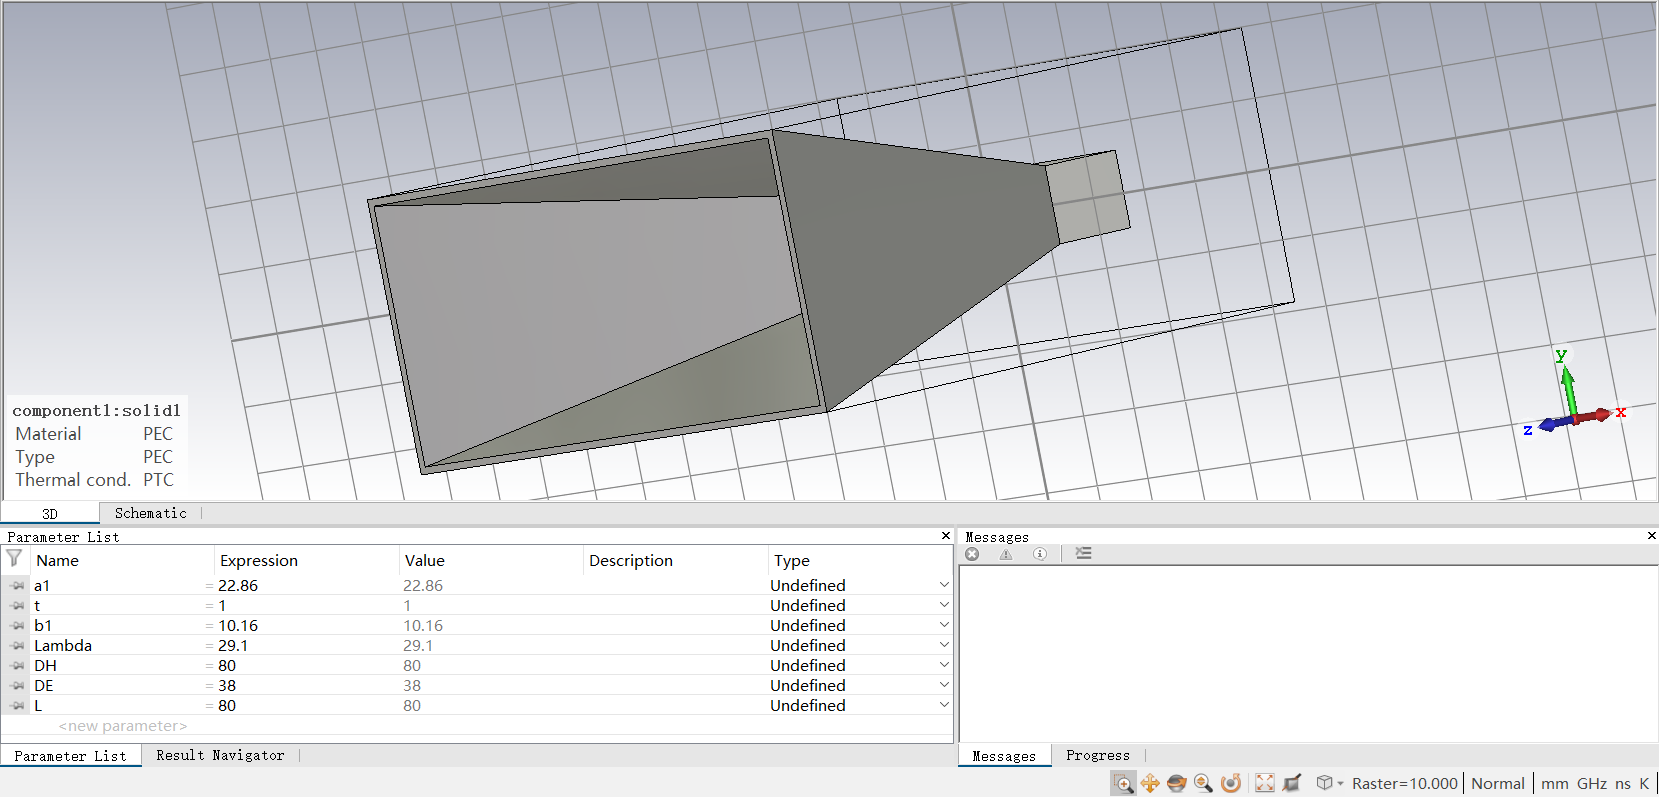
\includegraphics[width=\textwidth]{figures/矩形波导馈电的角锥喇叭天线 CST 模型.png}
        \caption{矩形波导馈电的角锥喇叭天线最终 CST 模型}
    \end{minipage}
    \label{fig:shell_build}
\end{figure}

\subsection*{3.3 仿真条件、端口与监视器设置}
完成物理模型的建立后，需要定义仿真的电磁环境及观测目标。具体设置步骤如下：

\begin{enumerate}
    \item \textbf{仿真频率与环境设置}：点击 \texttt{Simulation -> Frequency}，由于本实验天线工作在 X 波段，将频率范围设为 $8.2\,\text{GHz} \sim 12.4\,\text{GHz}$。在 \texttt{Background}（背景属性）中将周围环境材质设为 \texttt{Normal}（即真空/空气）。随后在 \texttt{Boundaries}（边界条件）中，将各方向的边界均设为 \texttt{open (add space)}，以模拟自由空间中的无反射辐射环境。以上设置分别如图16、图17和图18所示。
\end{enumerate}

\begin{figure}[htbp]
    \centering
    \begin{minipage}[t]{0.32\textwidth}
        \centering
        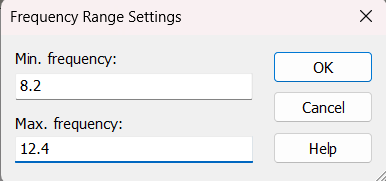
\includegraphics[width=\textwidth]{figures/频率设置.png}
        \caption{频率范围设置}
    \end{minipage}
    \hfill
    \begin{minipage}[t]{0.32\textwidth}
        \centering
        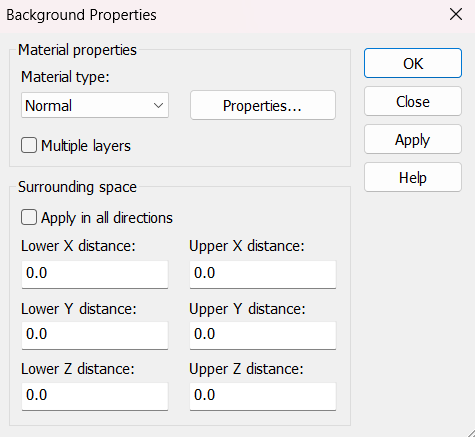
\includegraphics[width=\textwidth]{figures/背景设置.png}
        \caption{背景材料设置}
    \end{minipage}
    \hfill
    \begin{minipage}[t]{0.32\textwidth}
        \centering
        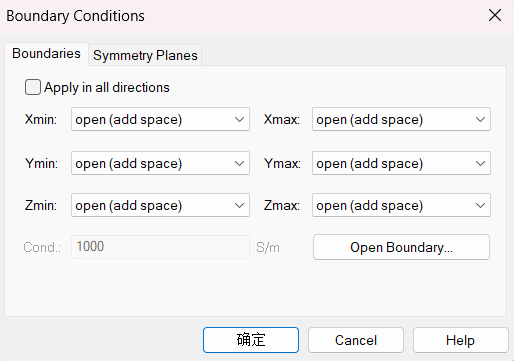
\includegraphics[width=\textwidth]{figures/边界设置.png}
        \caption{边界条件设置}
    \end{minipage}
    \label{fig:sim_env_settings}
\end{figure}

\begin{enumerate}
    \setcounter{enumi}{1}
    \item \textbf{端口设置}：选中波导的输入端面，执行 \texttt{Simulation -> Waveguide Port} 添加波导端口。为了在初步分析中观察高次模的情况，输入参数时将模式吸收数（\texttt{Number of modes}）暂时设置为 5。
    \item \textbf{场监视器设置}：点击 \texttt{Simulation -> Field Monitor}，分别添加频率为 $10.3\,\text{GHz}$ 的远场监视器（\texttt{Farfield/RCS}）、电场监视器（\texttt{E-Field}）以及表面电流监视器（\texttt{H-Field and Surface current}），以便在仿真结束后观察空间场分布及天线方向图。端口与监视器设置分别如图19、图20所示。
\end{enumerate}

\begin{figure}[htbp]
    \centering
    \begin{minipage}[t]{0.48\textwidth}
        \centering
        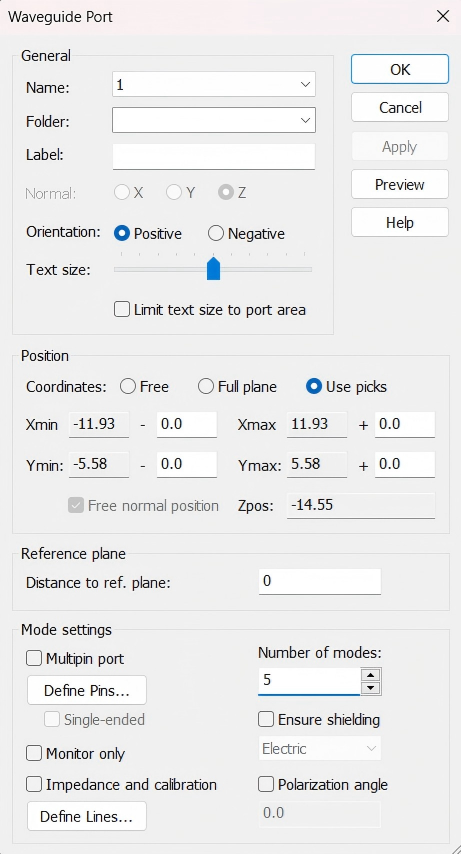
\includegraphics[width=\textwidth]{figures/端口设置.png}
        \caption{波导端口 (Port 1) 设置}
    \end{minipage}
    \hfill
    \begin{minipage}[t]{0.48\textwidth}
        \centering
        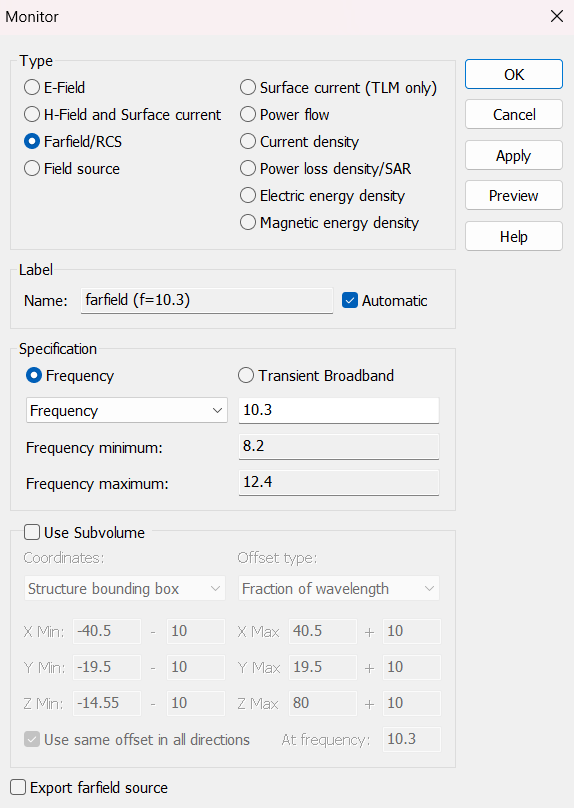
\includegraphics[width=\textwidth]{figures/监视器设置.png}
        \caption{电磁场监视器设置}
    \end{minipage}
    \label{fig:port_monitor_settings}
\end{figure}

\subsection*{3.4 端口模式分析与参数修正}
在进行全波时域仿真前，需先对波导端口传输的电磁波模式进行分析，以确定正确的激励模式数。

在时域求解器 \texttt{Simulation -> Setup Solver} 中，勾选 \texttt{Calculate port modes only}（仅计算端口模式）选项，执行 \texttt{Start}。计算完成后，打开 \texttt{Simulation -> Logfile -> Solve Logfile} 查看结果日志，设置与计算结果分别如图21、图22所示。

\begin{figure}[htbp]
    \centering
    \begin{minipage}[t]{0.48\textwidth}
        \centering
        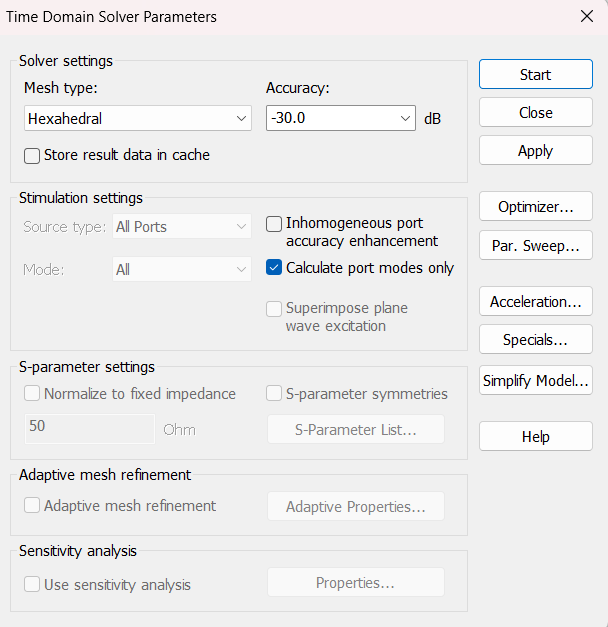
\includegraphics[width=\textwidth]{figures/TimeDomainParameters.png}
        \caption{端口模式分析设置选项}
    \end{minipage}
    \hfill
    \begin{minipage}[t]{0.48\textwidth}
        \centering
        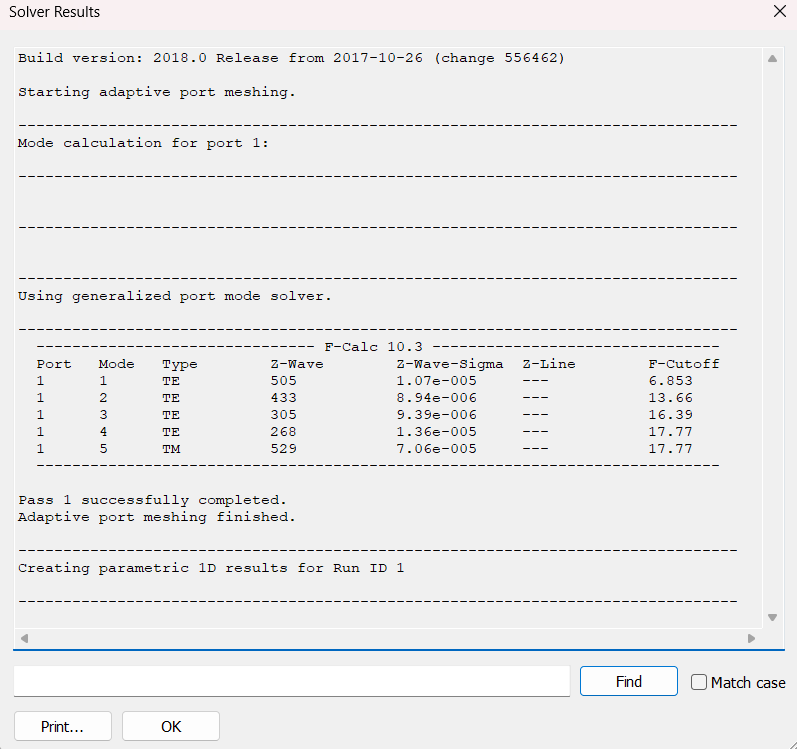
\includegraphics[width=\textwidth]{figures/SolverResults.png}
        \caption{求解器日志中的截止频率结果}
    \end{minipage}
    \label{fig:mode_analysis}
\end{figure}

\textbf{结果分析}：从日志计算结果可以看出，在波导端口截面处，模式 1（TE10 主模）的截止频率（\texttt{F-Cutoff}）为 $6.853\,\text{GHz}$，低于实验设置的最低频率 $8.2\,\text{GHz}$，能够顺利传输；而模式 2 的截止频率高达 $13.66\,\text{GHz}$，已经超出了仿真的最高工作频率 $12.4\,\text{GHz}$。

由此可以得出结论：由于仿真的最高频率为 $12.4\,\text{GHz}$，所以在该尺寸的喇叭天线结构中，其余高次模均处于截止状态，实际上只传输 $1$ 种模式的波（即主模）。因此，前置设置中要求吸收模式数大于 $1$ 只是为了验证此物理现象。

\textbf{参数修正}：明确传输模式后，为了进行正式的全空间辐射特性仿真，需再次打开 \texttt{Setup Solver}，取消勾选 \texttt{Calculate port modes only}。同时，将激励设置（\texttt{Stimulation settings}）修改为明确的 \texttt{Source type: Port 1} 且 \texttt{Mode: 1}。确认无误后点击 \texttt{Start}，开始正式的 3D 全波电磁仿真。

\makepart{实验结果和分析处理}

\subsection*{4.1 喇叭天线端口阻抗匹配特性分析 (S11 与 VSWR)}
在 CST 全波时域仿真完成后，通过提取端口 1 的 1D Results，可以得到反映天线阻抗匹配性能的两个核心指标曲线：S11（反射系数幅度）与 VSWR（电压驻波比），分别如图23、图24所示。

\begin{figure}[htbp]
    \centering
    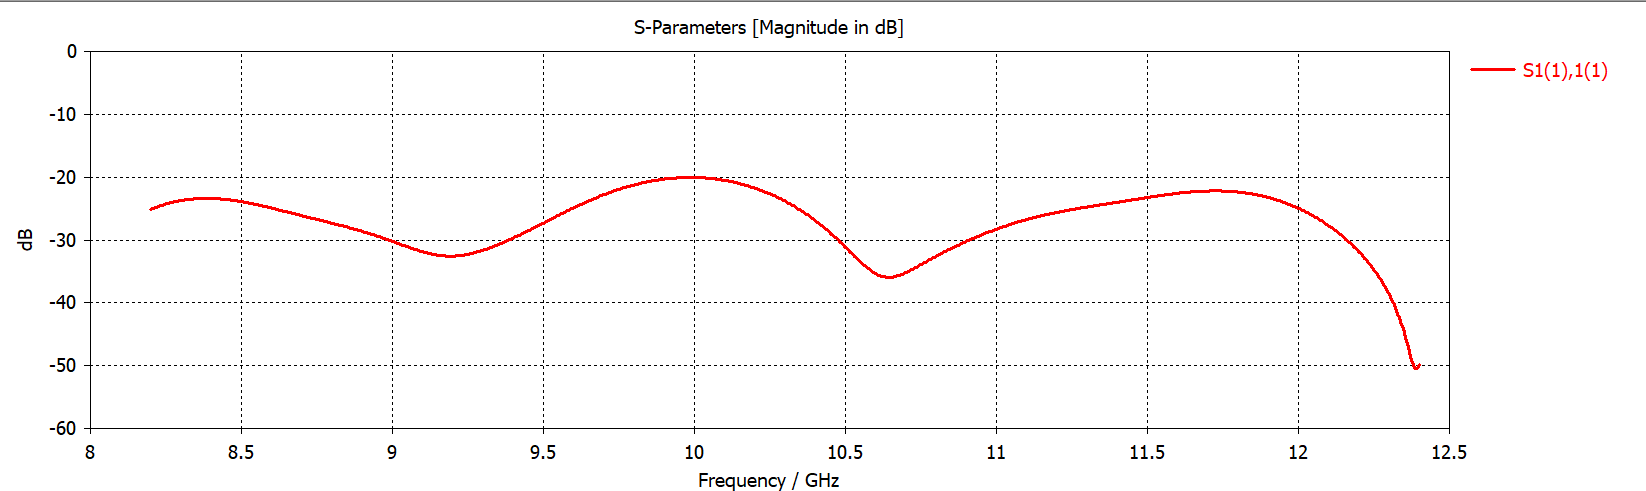
\includegraphics[width=0.85\textwidth]{figures/S11.png}
    \caption{角锥喇叭天线 S11 特性曲线}
    \label{fig:s11}
\end{figure}

\begin{figure}[htbp]
    \centering
    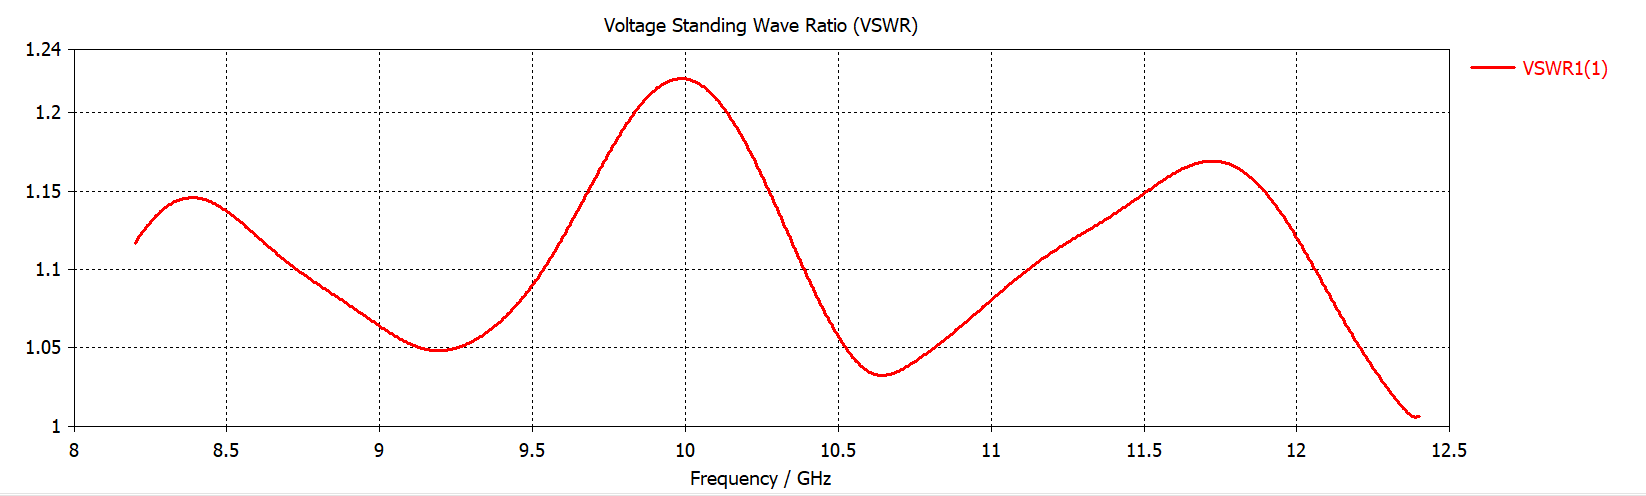
\includegraphics[width=0.85\textwidth]{figures/VSWR.png}
    \caption{角锥喇叭天线 VSWR 特性曲线}
    \label{fig:vswr}
\end{figure}

\textbf{数据分析与结论：}
\begin{itemize}
    \item \textbf{S11 特性分析}：从 S11 曲线图中可以看出，在 $8.2\,\text{GHz} \sim 12.4\,\text{GHz}$ 的整个 X 波段工作频率范围内，天线主模的反射系数幅度均保持在 $-20\,\text{dB}$ 左右及以下波动，且在 $12.4\,\text{GHz}$ 附近取得极小值（下探至约 $-50\,\text{dB}$）。这说明从波导端口馈入的电磁波能量极少被反射回波导中，天线端口具有极佳的能量传输效率。
    \item \textbf{VSWR 特性分析}：电压驻波比（VSWR）与 S11 在物理意义上相互对应，用于衡量馈线内部形成驻波的严重程度（理想完全匹配状态下 VSWR 为 1）。从图中可以看出，在整个工作频段内，该天线的最大驻波比仅为 1.23 左右（位于 $10\,\text{GHz}$ 频点附近），其余大部分频点均在 1.1 左右。这远优于微波工程中通常要求的 VSWR $< 2$（甚至 $< 1.5$）的合格标准。
    \item \textbf{综合评价}：上述极其理想的 S11 和 VSWR 数据充分验证了实验原理中的理论推导——角锥喇叭由波导逐渐平滑扩展的几何结构，起到了非常优秀的阻抗变换器作用，成功实现了矩形波导特性阻抗与自由空间波阻抗的宽带良好匹配。
\end{itemize}

\subsection*{4.2 喇叭天线辐射方向图与增益特性分析}
为了全面评估角锥喇叭天线的空间辐射特性，本实验提取了中心频率为 $10.3\,\text{GHz}$ 时的 3D 远场辐射方向图，以及 E 面（垂直面，$\Phi=90^\circ$）和 H 面（水平面，$\Phi=0^\circ$）的 2D 极坐标切面图，分别如图 \ref{fig:3d_pattern}、图 \ref{fig:e_plane} 和图 \ref{fig:h_plane} 所示。

\begin{figure}[htbp]
    \centering
    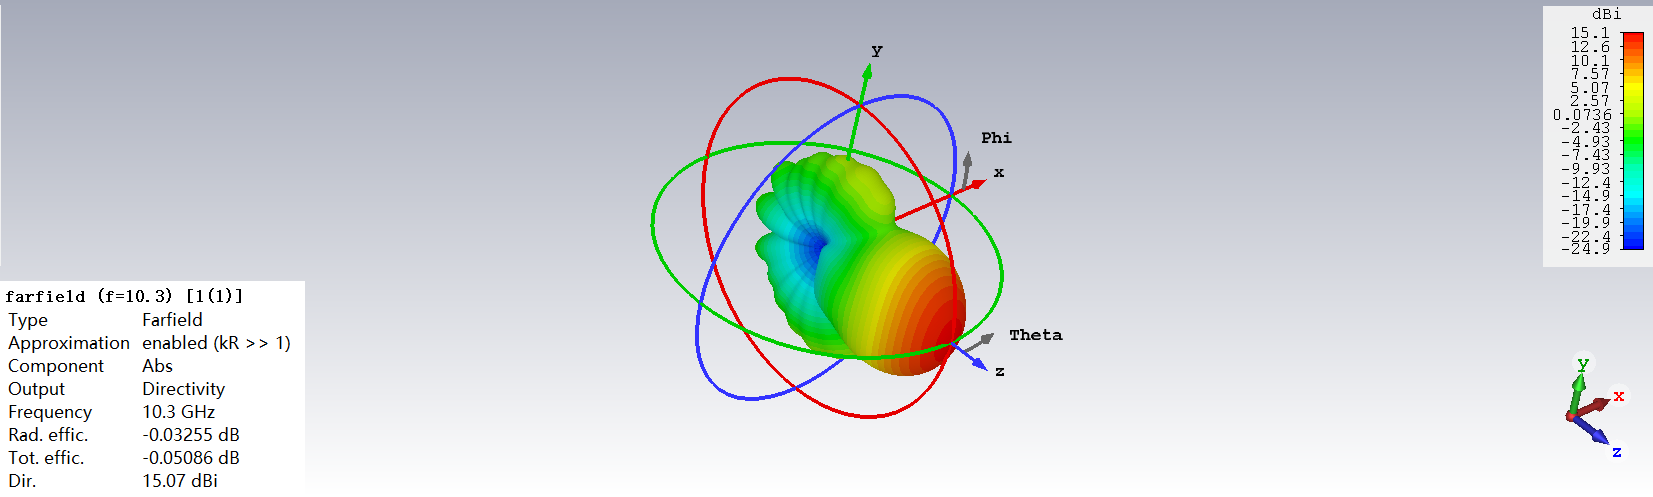
\includegraphics[width=0.7\textwidth]{figures/方向图.png}
    \caption{中心频率 10.3 GHz 下的 3D 远场辐射方向图}
    \label{fig:3d_pattern}
\end{figure}

\begin{figure}[htbp]
    \centering
    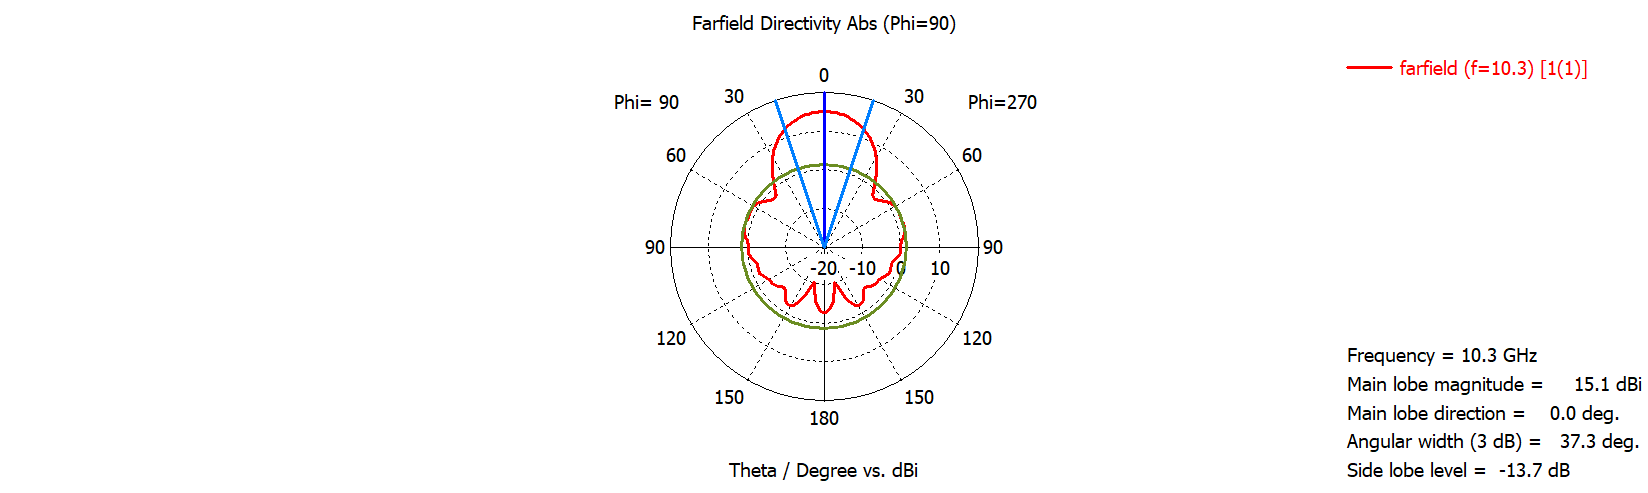
\includegraphics[width=0.85\textwidth]{figures/90方向图.png}
    \caption{角锥喇叭天线 E 面 (垂直面, $\Phi=90^\circ$) 极坐标方向图}
    \label{fig:e_plane}
\end{figure}

\begin{figure}[htbp]
    \centering
    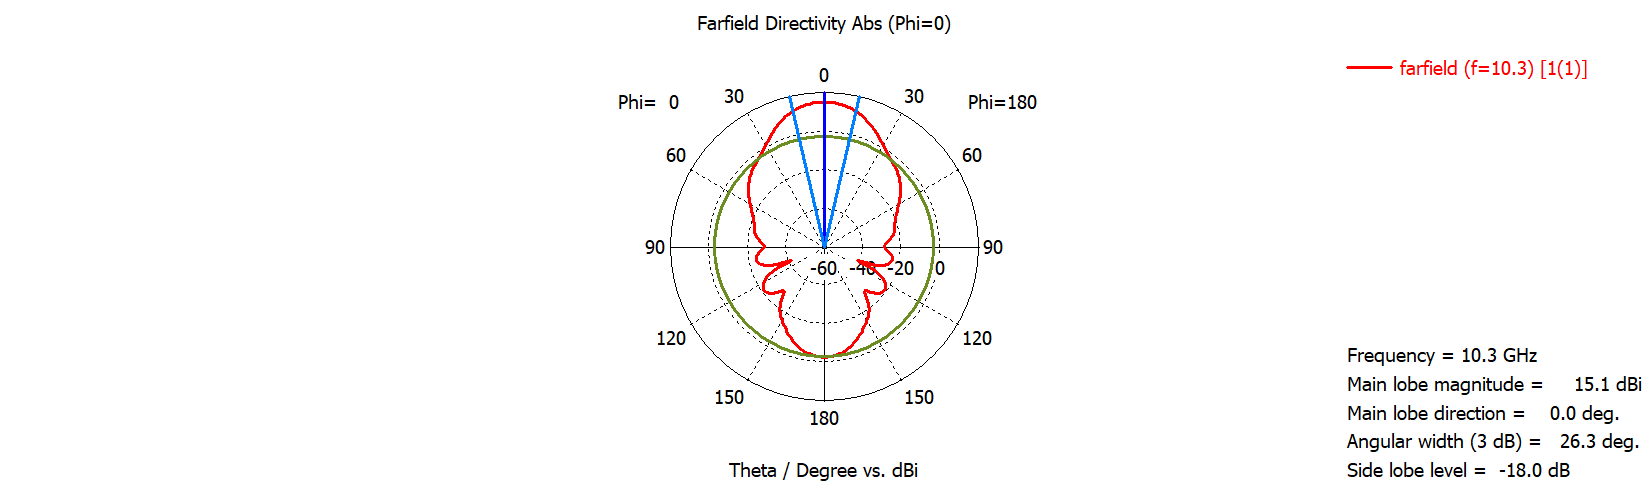
\includegraphics[width=0.85\textwidth]{figures/0方向图.png}
    \caption{角锥喇叭天线 H 面 (水平面, $\Phi=0^\circ$) 极坐标方向图}
    \label{fig:h_plane}
\end{figure}

\textbf{仿真数据提取与对比分析：}
\begin{itemize}
    \item \textbf{3D 辐射特性与增益对比}：由图 \ref{fig:3d_pattern} 可知，天线的主辐射方向沿 $Z$ 轴正方向分布，能量高度集中。由于该模型采用理想导体（PEC）材质且阻抗匹配极佳，辐射效率接近 100%，因此其最大方向性系数（$15.07\,\text{dBi}$）近似等于其实际增益。该仿真增益值与我们在实验原理中通过半经验公式计算出的理论增益（约 $16.05\,\text{dB}$）十分接近。误差主要来源于理论公式中对口径面相位分布所做的近似假设，这在工程允许的合理误差范围之内。
    
    \item \textbf{E 面（垂直面）辐射特性}：如图 \ref{fig:e_plane} 所示，E 面方向图的主瓣方向准确指向 $0^\circ$（正前方），其半功率波瓣宽度（3dB Angular width）为 $37.3^\circ$，第一副瓣电平（Side lobe level）为 $-13.7\,\text{dB}$。
    
    \item \textbf{H 面（水平面）辐射特性}：如图 \ref{fig:h_plane} 所示，H 面方向图的主瓣同样指向 $0^\circ$，其半功率波瓣宽度为 $26.3^\circ$，第一副瓣电平为 $-18.0\,\text{dB}$。
    
    \item \textbf{综合理论评价}：对比 E 面与 H 面的 2D 极坐标图数据可以发现，H 面的波瓣宽度（$26.3^\circ$）明显窄于 E 面的波瓣宽度（$37.3^\circ$）。这一仿真结果完美契合了天线的物理结构特征：本实验中角锥喇叭的 H 面口径尺寸（$D_H = 80\,\text{mm}$）大于 E 面口径尺寸（$D_E = 38\,\text{mm}$）。根据天线原理，有效口径尺寸越大的平面，其聚焦能力越强，波束也就越窄。此外，较低的副瓣电平（$-13.7\,\text{dB}$ 与 $-18.0\,\text{dB}$）也证明了该天线具有优良的定向辐射性能，漏射能量极小。
\end{itemize}

\subsection*{4.3 理论增益与仿真结果的对比分析}
为了验证角锥喇叭天线设计的准确性，将 CST 仿真得到的增益（Gain）结果与 2.3 节中的理论计算值进行交叉印证。仿真得到的 3D 增益及二维极坐标切面增益分别如图 \ref{fig:3d_gain}、图 \ref{fig:e_gain} 和图 \ref{fig:h_gain} 所示。

\begin{figure}[htbp]
    \centering
    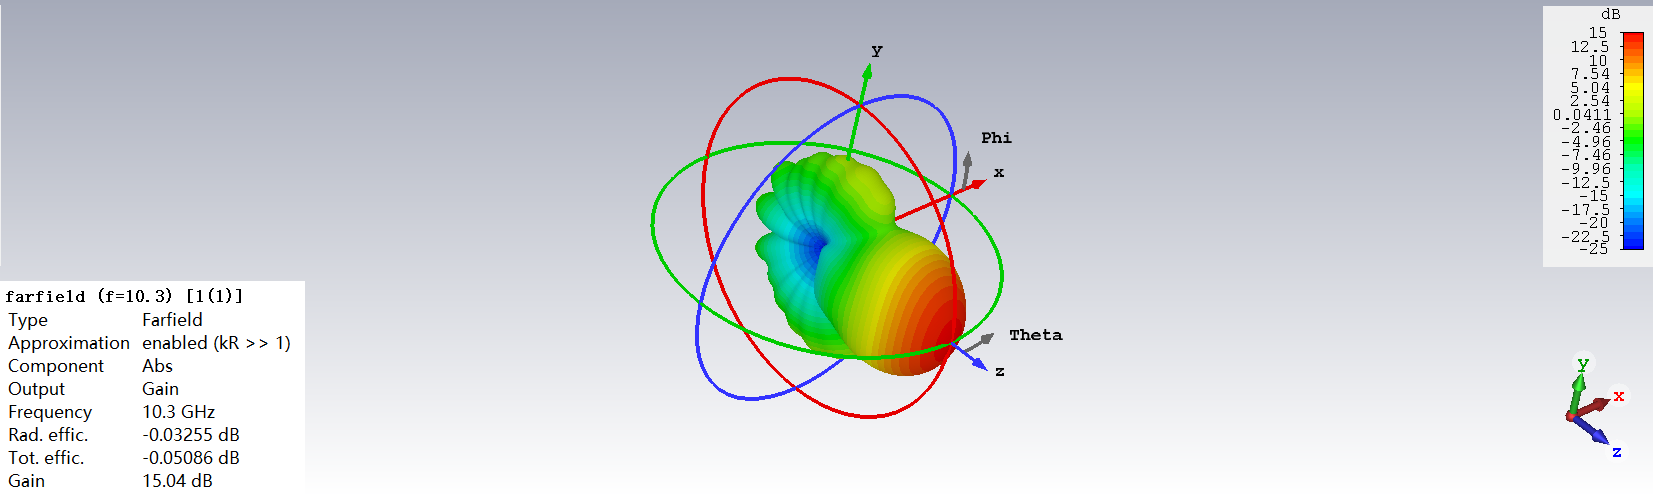
\includegraphics[width=0.7\textwidth]{figures/增益.png}
    \caption{中心频率 10.3 GHz 下的 3D 远场增益分布图}
    \label{fig:3d_gain}
\end{figure}

\begin{figure}[htbp]
    \centering
    \begin{minipage}[t]{0.48\textwidth}
        \centering
        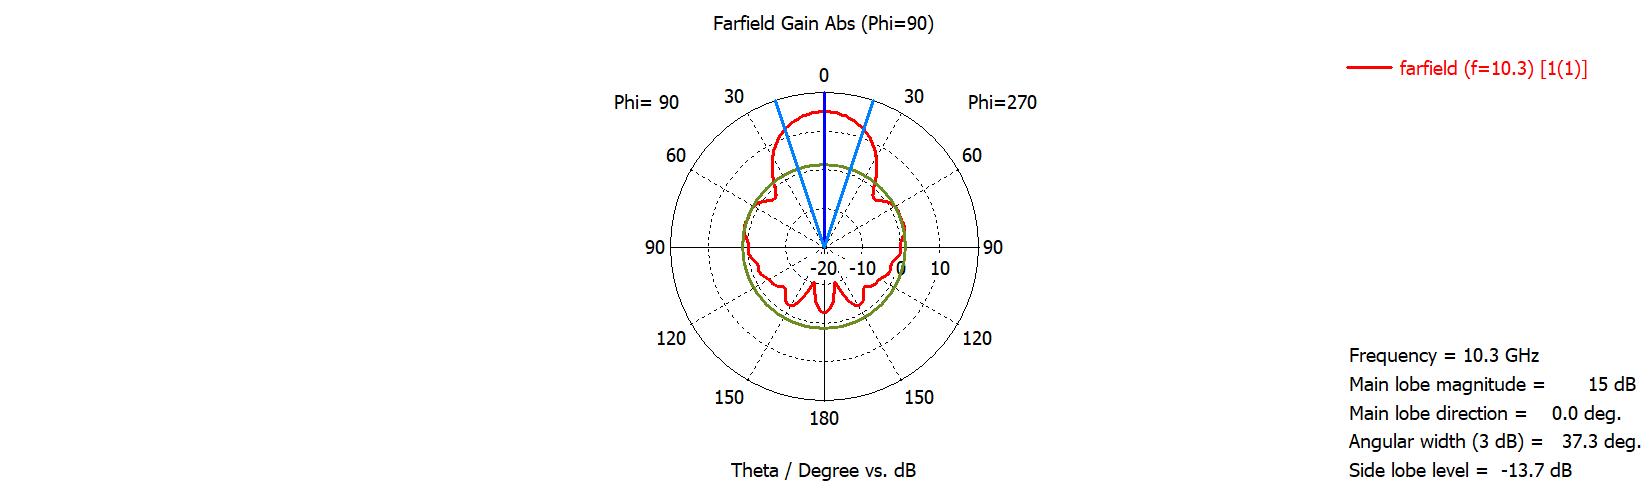
\includegraphics[width=\textwidth]{figures/90增益.png}
        \caption{E 面 ($\Phi=90^\circ$) 极坐标增益图}
        \label{fig:e_gain}
    \end{minipage}
    \hfill
    \begin{minipage}[t]{0.48\textwidth}
        \centering
        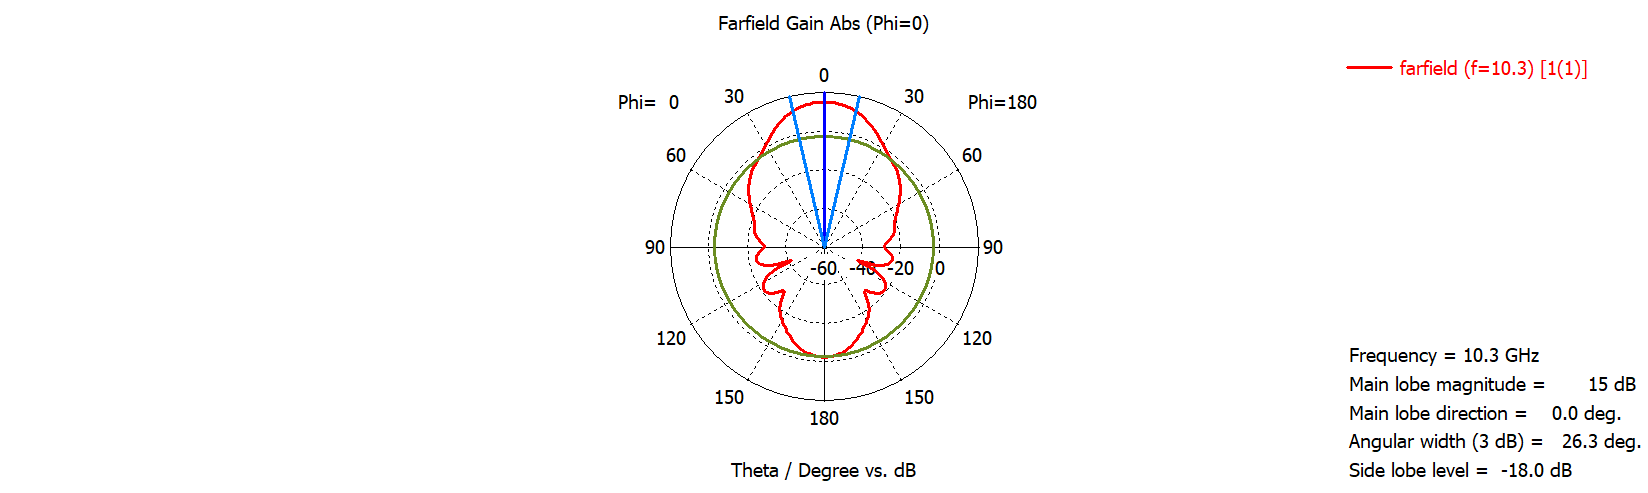
\includegraphics[width=\textwidth]{figures/0增益.png}
        \caption{H 面 ($\Phi=0^\circ$) 极坐标增益图}
        \label{fig:h_gain}
    \end{minipage}
\end{figure}

\textbf{1. 理论增益计算}

根据 2.3 节的增益理论计算公式 (1) 及天线几何参数（$D_H = 80\,\text{mm}, D_E = 38\,\text{mm}, L = 80\,\text{mm}, \lambda = 29.1\,\text{mm}$），可求得口径面积 $A^2 = 3040\,\text{mm}^2$。
经计算相差参数 $\alpha \approx 0.88, \beta \approx 0.94$，查表得到由于口径相位不均匀引起的增益衰减因子 $\Delta G_H \approx 0.088\,\text{dB}, \Delta G_E \approx 0.21\,\text{dB}$。
代入公式，得出该角锥喇叭天线的理论增益近似为：
$$G \approx 10.8 + 10\lg\left(\frac{3040}{29.1^2}\right) - 0.088 - 0.21 \approx 16.05\,\text{dB}$$

\textbf{2. 仿真结果与理论值的异同点分析}
\begin{itemize}
    \item \textbf{相同点（趋势一致性）}：如图 \ref{fig:3d_gain} 所示，CST 仿真得到的最大增益为 $15.04\,\text{dB}$，这与理论计算的 $16.05\,\text{dB}$ 在数值量级上高度吻合，证明了天线尺寸设计的合理性。此外，增益图的波瓣宽度（E 面 $37.3^\circ$，H 面 $26.3^\circ$）与 4.2 节中的方向性系数图完全对应，再次验证了该模型极高的辐射效率。
    \item \textbf{不同点（数值差异）}：仿真增益（$15.04\,\text{dB}$）略低于理论估算增益（$16.05\,\text{dB}$），存在约 $1\,\text{dB}$ 左右的数值误差。
    \item \textbf{误差来源深度分析}：
    \begin{enumerate}
        \item \textbf{理论公式的理想化假设}：2.3 节中的半经验理论公式是基于理想的口径场分布（假设振幅按 $TE_{10}$ 模标准余弦分布，相位呈严格二次方非线性分布）推导得出的。而在实际的 CST 全波仿真中，喇叭口径边缘必然存在电磁波的\textbf{边缘绕射效应（Edge Diffraction）}，这些绕射场会干涉主辐射场，导致实际增益略有下降。
        \item \textbf{相心不完全重合损耗}：由于该喇叭天线的尺寸是根据给定的波导尺寸进行直接扩展，其 H 面和 E 面展开的虚顶点（$R_1$ 和 $R_2$）在物理几何上并未达到完美的重合状态。这种非最佳喇叭结构会导致口径面上的等相位面发生轻微畸变，从而引起实际增益的轻微衰减。
        \item \textbf{查表与计算插值误差}：在理论计算环节，参数 $\Delta G_H$ 和 $\Delta G_E$ 是通过离散数值表进行线性插值获取的近似值，数学估算本身也会引入一定的截断误差。
    \end{enumerate}
\end{itemize}

\subsection*{4.4 喇叭天线与波导端口的电磁场分布分析}
为了直观地理解电磁波在波导和喇叭天线中的传输与辐射机理，本节对波导端口的模式场分布以及天线整体的空间场分布进行了提取与分析。

\textbf{1. 波导端口的初始电磁场分布 (Port Modes)}

在馈电矩形波导端口处，提取计算得到的电场（e1）和磁场（h1）矢量分布，分别如图 \ref{fig:port_e1} 和图 \ref{fig:port_h1} 所示。

\begin{figure}[htbp]
    \centering
    \begin{minipage}[t]{0.48\textwidth}
        \centering
        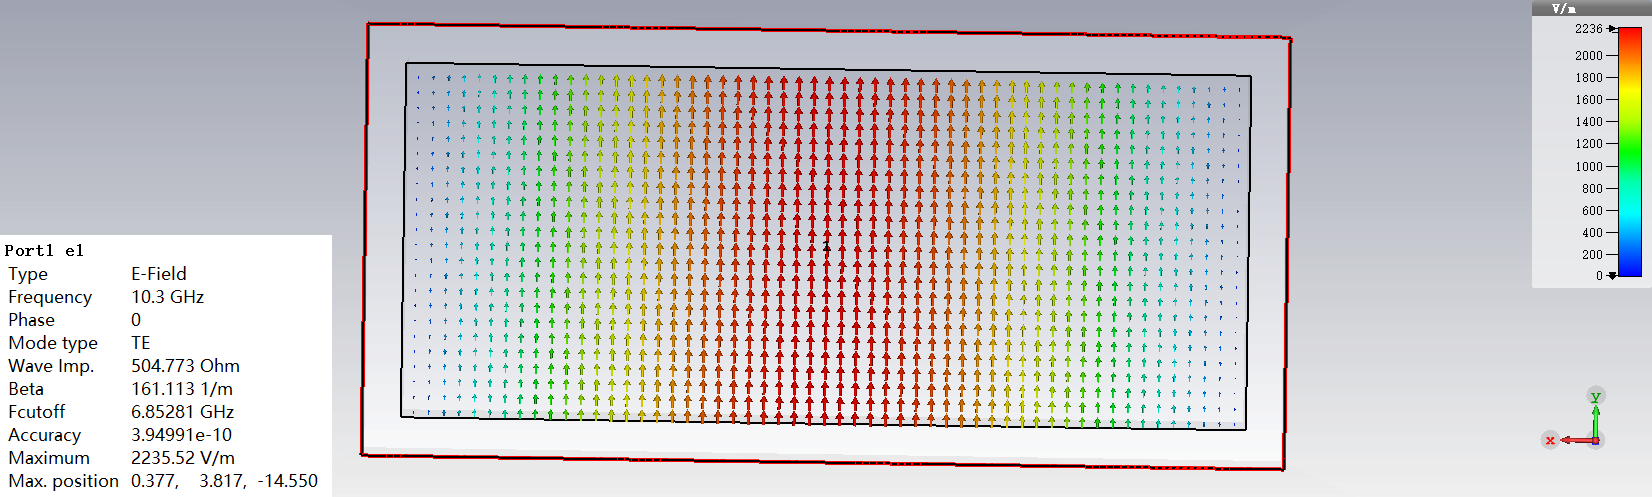
\includegraphics[width=\textwidth]{figures/e1.png}
        \caption{波导端口的电场分布 (e1)}
        \label{fig:port_e1}
    \end{minipage}
    \hfill
    \begin{minipage}[t]{0.48\textwidth}
        \centering
        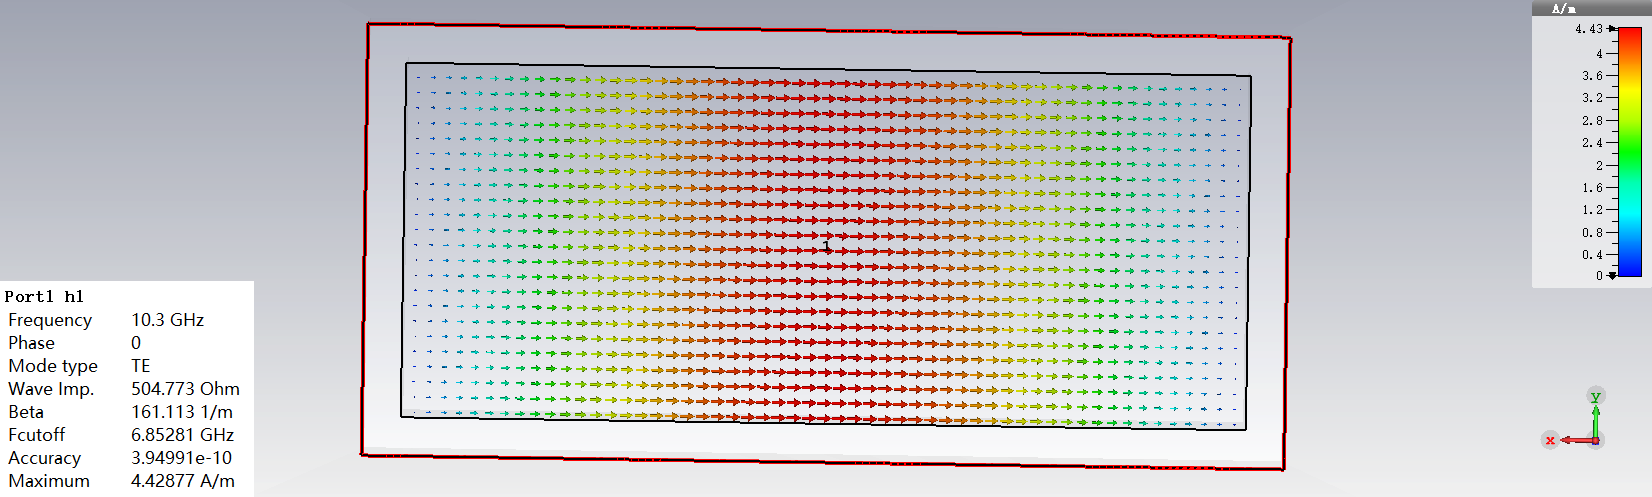
\includegraphics[width=\textwidth]{figures/h1.png}
        \caption{波导端口的磁场分布 (h1)}
        \label{fig:port_h1}
    \end{minipage}
\end{figure}

\textbf{分析}：由图可见，波导端口的电场矢量方向严格平行于矩形波导的窄边（Y轴），且在宽边（X轴）中心处电场强度最大，向两侧边缘逐渐递减至零；而磁场矢量则呈现出环绕电场的闭合回路线。这完美地呈现了矩形波导中 $\text{TE}_{10}$ 主模的典型场分布特征，证明了端口激励设置的绝对正确。

\textbf{2. 天线整体空间电磁场与表面电流分布}

利用 3D 场监视器提取中心频率 $10.3\,\text{GHz}$ 下的空间电场、磁场以及金属表面的电流分布，分别如图33、图34及图35、图36所示。

\begin{figure}[htbp]
    \centering
    \begin{minipage}[t]{0.48\textwidth}
        \centering
        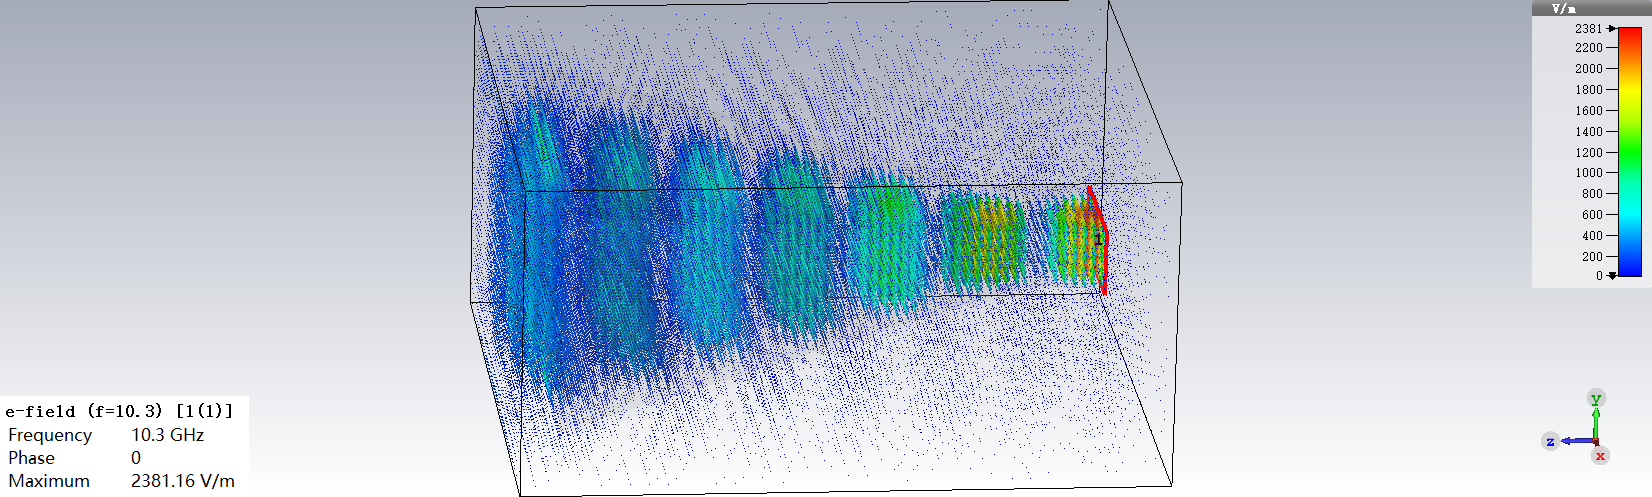
\includegraphics[width=\textwidth]{figures/电场.png}
        \caption{喇叭天线内部的空间电场传播分布}
    \end{minipage}
    \hfill
    \begin{minipage}[t]{0.48\textwidth}
        \centering
        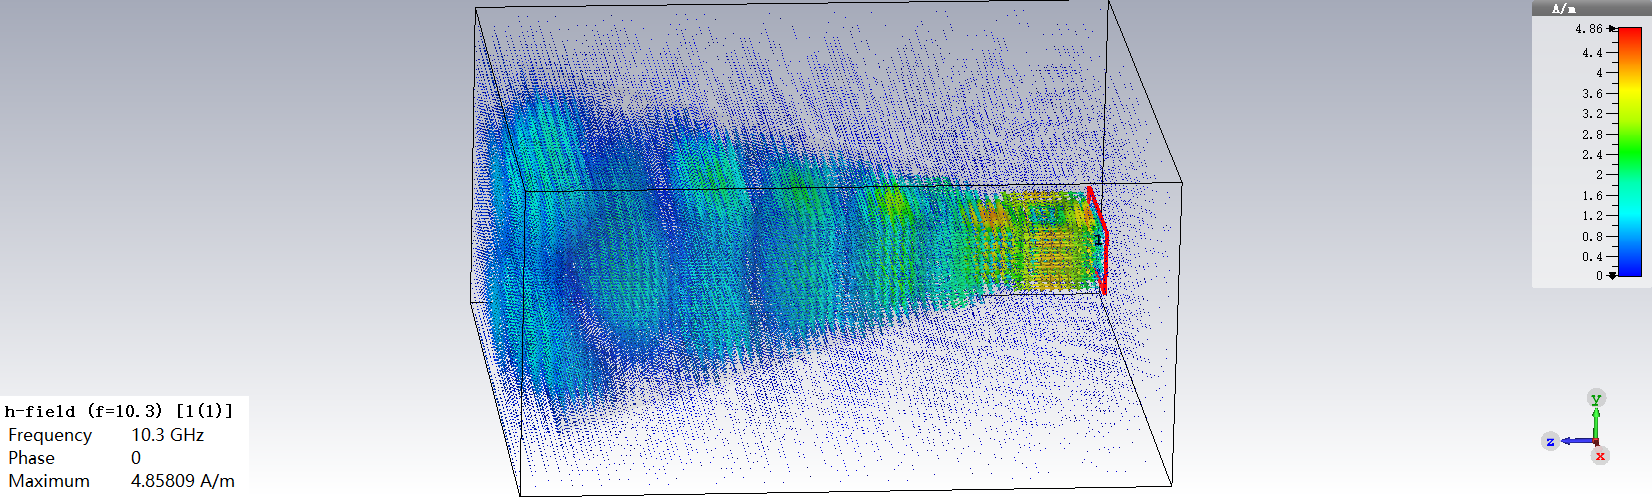
\includegraphics[width=\textwidth]{figures/磁场.png}
        \caption{喇叭天线内部的空间磁场传播分布}
    \end{minipage}
    \label{fig:field_3d}
\end{figure}

\begin{figure}[htbp]
    \centering
    \begin{minipage}[t]{0.48\textwidth}
        \centering
        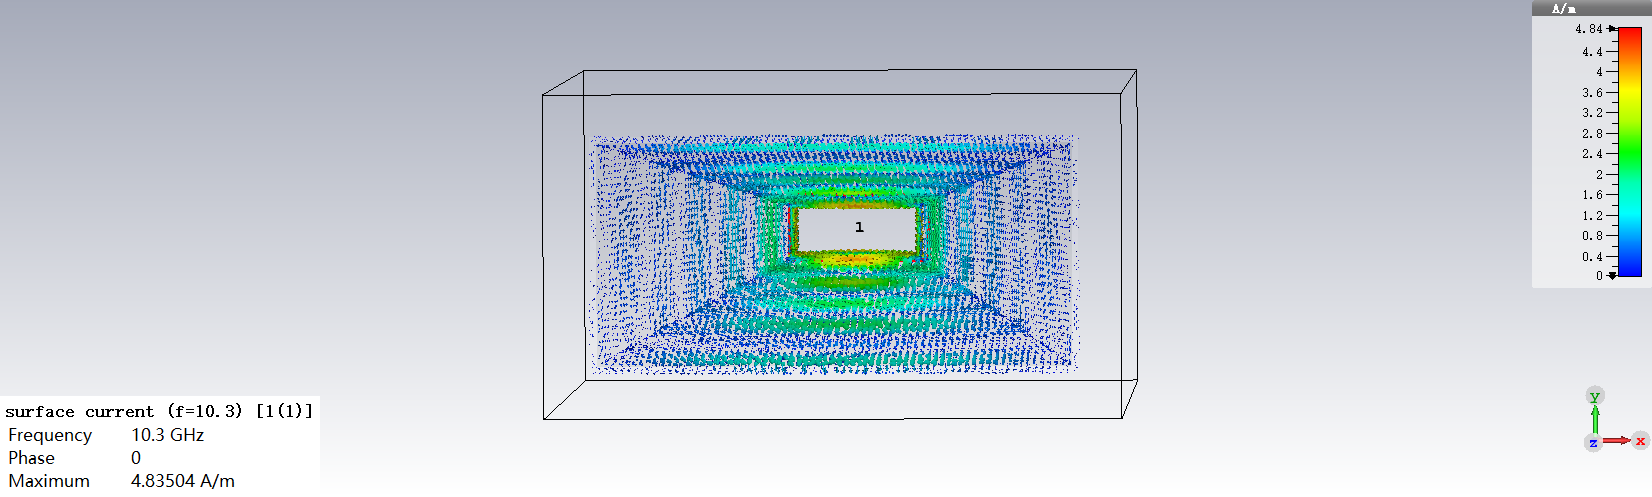
\includegraphics[width=\textwidth]{figures/表面电流内部.png}
        \caption{喇叭天线表面电流分布 (内部视角)}
    \end{minipage}
    \hfill
    \begin{minipage}[t]{0.48\textwidth}
        \centering
        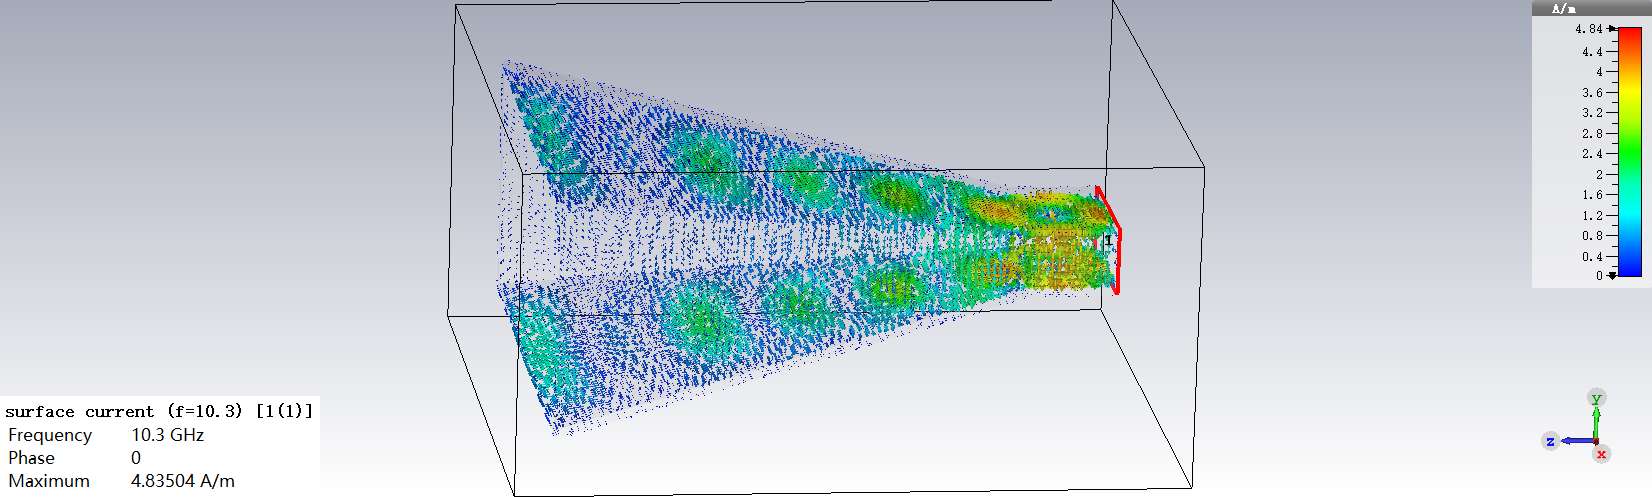
\includegraphics[width=\textwidth]{figures/表面电流外部.png}
        \caption{喇叭天线表面电流分布 (外部视角)}
    \end{minipage}
    \label{fig:surface_current}
\end{figure}

\textbf{分析}：从图33和图34中可以清晰地观察到，当 $\text{TE}_{10}$ 模电磁波从等截面的矩形波导进入渐变扩展的角锥喇叭区域后，其等相位面逐渐从平面波转变为球面波，并在喇叭口径处挣脱金属壁的束缚，向自由空间辐射。从图35和图36的表面电流分布可以看出，高强度的传导电流主要集中在波导内壁及喇叭的喉部区域，随着截面积的逐渐增大，电流密度在喇叭侧壁上逐渐稀疏并呈现出驻波与行波交织的分布形态。

\subsection*{4.5 实验结论}
综合本次电磁场与电磁波 CST 仿真实验的全流程数据，得出以下结论：

从仿真结果来看，该矩形波导馈电的角锥喇叭天线的主瓣辐射方向为 $\theta=0^\circ, \phi=0^\circ$（正前方），其 E 面（垂直面）和 H 面（水平面）的半功率波瓣宽度分别为 $37.3^\circ$ 和 $26.3^\circ$，最大定向增益达到了 $15.04\,\text{dB}$，该最大增益的仿真值与理论估算值（$16.05\,\text{dB}$）非常相近。同时，该天线输入端口的反射系数（S11）在 $8.2\,\text{GHz} \sim 12.4\,\text{GHz}$ 的整个 X 波段工作频段内均保持在 $-20\,\text{dB}$ 以下，最大驻波比（VSWR）仅为 1.23，表现出了极其优异的宽带阻抗匹配性能，能够非常高效地工作。

虽然仿真结果中由于边缘绕射等非理想因素的存在，与绝对理论推导值有轻微的偏差，但这反而体现了实际工程设计的真实物理情况。通过本次 CST 建模与仿真，我们不仅直观、透彻地掌握了矩形波导馈电的角锥喇叭天线的内部电磁场传播规律，更深刻验证了其优良的定向辐射特性。实验圆满达到了预期目的。

\makepart{实验收获与体会}

\subsection*{5.1 CST 电磁仿真工具的熟练掌握}
通过本次角锥喇叭天线的建模与仿真实验，我最直观的收获是掌握了 CST Studio Suite 这一工业级仿真软件的完整工作流。
\begin{itemize}
    \item \textbf{参数化建模的优越性}：在实验初期，我深刻体会到了参数化建模（Parameter List）的重要性。通过定义变量而非固定数值，我不仅能快速修改天线尺寸，更理解了参数化设计对于工程优化和系列化产品设计的核心意义。
    \item \textbf{从求解器到监视器的逻辑链}：我学会了如何根据仿真目标（如宽带匹配或单频点辐射）正确设置频率范围、边界条件以及远场/电场监视器。尤其是通过“模式分析（Calculate port modes only）”来验证波导高次模的截止，让我对仿真软件的内在逻辑有了更深的认识。
\end{itemize}

\subsection*{5.2 对《电磁场与电磁波》理论课的极大助力}
长期以来，电磁场理论中的矢量运算、波动方程以及边界条件相对抽象，而本次仿真实验将这些“纸面公式”转化为了“可视化图景”，对我理解理论课程帮助极大：
\begin{itemize}
    \item \textbf{电磁波模式的具象化}：在观察 $\text{TE}_{10}$ 模的端口分布时，我第一次清晰地看到了电场强度在宽边中心最强、边缘为零的余弦分布规律，这比课本上的 2D 图形要生动得多。
    \item \textbf{波导截止特性的验证}：通过查看求解器日志（Logfile），我亲手验证了主模与高次模截止频率的计算过程。当看到模式 2 的截止频率确实超出了工作频段时，我对“单模传输”这一概念有了物理层面的把握。
    \item \textbf{阻抗匹配与辐射机理}：通过调节 S11 量程并观察 S 参数曲线，我理解了喇叭天线如何通过渐变结构实现波导与自由空间的阻抗变换。看到电磁波平滑地从波导辐射出去，我才真正理解了“阻抗匹配”在微波系统中的核心地位。
\end{itemize}

\subsection*{5.3 工程素养与误差分析能力的提升}
本次实验也锻炼了我作为准工程师的独立思考能力：
\begin{itemize}
    \item \textbf{严谨的数据对比分析}：在比较 $15.04\,\text{dB}$（仿真值）与 $16.05\,\text{dB}$（理论值）的差异时，我没有简单地得出“实验失败”或“软件不准”的结论，而是深入探讨了理论公式中关于口径面相位的理想化假设。这种对误差来源（如边缘绕射、相心不重合等）的深入剖析，是我在纯理论学习中难以获得的。
    \item \textbf{排障与调试的耐心}：在实验过程中，我也遇到过忘记添加监视器导致没有彩图、或者是参数设置报错的情况。通过查阅手册和反复尝试，我意识到仿真不仅是“跑个结果”，更是对物理模型不断修正和精细化处理的过程。
\end{itemize}

\textbf{结语}：
本次实验是我从理论学习向科研实践迈出的重要一步。它让我明白，优秀的软件操作是基础，而深厚的理论功底才是指导仿真、分析结果的“灯塔”。在未来的专业课程学习中，我将更多地尝试利用仿真工具辅助理论推导，实现知行合一。

\end{document}
